\documentclass[a4paper,12pt]{article}
%\usepackage declarations should go here
\usepackage{graphicx}
\usepackage[T
1]{fontenc}
\usepackage{parskip}
\usepackage{latexsym,amsmath,amssymb}
\usepackage{natbib}
\usepackage{times}
\usepackage{zi4}
\usepackage[a4paper,left=3cm,right=3cm,top=3cm,bottom=3cm]{geometry}
%\usepackage{foundrysterlingbookosf}


% Turn off page numbering until first section.
\pagenumbering{gobble}
\usepackage[utf8]{inputenc}
\usepackage{tikz-cd}
\usepackage{biblatex}
\usepackage{amsmath}
\addbibresource{refs.bib}
\usepackage{multirow}
\usepackage{subcaption}
\usepackage{mwe}
\usepackage{caption}
\usepackage{multirow}
\usepackage{booktabs}
\usepackage[normalem]{ulem}
\DeclareMathOperator*{\argmax}{arg\,max}
\DeclareMathOperator*{\argmin}{arg\,min}
\usepackage{xcolor}
\usepackage{wrapfig}
\usepackage{hyperref}
\usepackage{threeparttable}
\usetikzlibrary{decorations.pathreplacing}
\usetikzlibrary{positioning}
\captionsetup[table]{labelfont=bf}
\captionsetup[figure]{labelfont=bf}
\usepackage{longtable}
\usetikzlibrary{shapes,decorations,arrows,calc,arrows.meta,fit,positioning}
\tikzset{
    -Latex,auto,node distance =1 cm and 1 cm,semithick,
    state/.style ={ellipse, draw, minimum width = 0.7 cm},
    point/.style = {circle, draw, inner sep=0.04cm,fill,node contents={}},
    bidirected/.style={Latex-Latex,dashed},
    el/.style = {inner sep=2pt, align=left, sloped}
}
% credit: https://dkumor.com/posts/technical/2018/08/15/causal-tikz/
\usetikzlibrary{shapes.geometric, arrows.meta, positioning, decorations.pathreplacing}
\author{Salim Damerdji}
\date{August 2023}

\begin{document}
\begin{titlepage}
\begin{center}
\vspace{1cm}
\textsf{\Huge{University of Oxford \\}}
\vspace{1cm}
\begin{figure}[htb]
\centering

\includegraphics[scale=.8]{figures/stats_logo.jpg}
\end{figure}
\vspace{2.0cm}
\Huge{How much housing will get built in San Francisco if building housing costs less?\\}
\vspace{2.0cm}
\large{ by \\[14pt] Salim Damerdji \\[8pt] Green Templeton College} \\
\vspace{2.2cm}
\large{A dissertation submitted in partial fulfilment of the degree of Master of
Science in Applied Statistics.
} \\
\vspace{.5cm}
\large{\emph{Department of Statistics, 24--29 St Giles, \\Oxford, OX1 3LB}} \\
\vspace{1.0cm}
\large{September 2023} \\
\end{center}
\end{titlepage}
\clearpage
This is my own work (except where otherwise indicated)
\vspace{2.5in}
\begin{center}
Candidate: Salim Damerdji\\
\vspace{1.0in}
Signed:.................................\\
\vspace{1.0in}
Date:...................................
\end{center}
\clearpage
% Here is the abstract.
\begin{abstract}
\noindent To end California's housing shortage, policymakers at the local and state level pass bills that reduce the cost of building homes, but policymakers remain in the dark as to how many more homes will be built as a result of their interventions to reduce the cost of building. To fill this gap in public policy research, I construct a novel panel dataset with N=1,531,273 observations of n=153,207 plots of land spanning T=10 years of San Francisco's housing market. To identify the partial effect of the cost of homebuilding on housing production, I use accidental fires as an instrumental variable. I then compare this estimate to the estimated averaged treatment effect in a geospatial regression discontinuity where I exploit geospatial discontinuities in how San Francisco levies fees on proposed residential development.

\end{abstract}
%----
\clearpage
%\thispagestyle{empty}
\vspace*{2in}
\begin{center}
\textbf{Acknowledgements}
\end{center}
I would like to thank Professor Frank Windmeijer for his supererogatory support, thoughtful feedback, and kind open-door policy. Spending time learning with Professor Frank Windmeijer was a highlight of my time studying at Oxford.
\clearpage
\tableofcontents
\listoffigures
\listoftables
\clearpage
\pagenumbering{arabic}

\section{Introduction}

Due to California's housing shortage,\cite{alamo2015california} policy researchers routinely try to estimate how proposed housing policies will impact the number of homes built per year in California.\cite{metcalf2021will}\cite{ab2011}\cite{la} 

A solution to this problem rests in the fact that policy researchers have a strong prior regarding how new laws impact the economic return of building housing.\cite{metcalf2021will}\cite{ab2011}\cite{la} If we also knew the causal effect of such returns on housing production, we could then estimate the indirect supply effects of new legislation. This dissertation aims to evaluate how housing production is driven by changes in the economic return of residential development. 

Policymakers in California care about the impact of housing legislation on ending the state's housing shortage. 

In the general case, policymakers would like to know the supply effects of regulatory changes that may never have been enacted anywhere before. This limits the usefulness of causal analyses of observational data. Furthermore, even where this observational data exists elsewhere, external validity issues arise.

In this report, I first propose a financial metric $D$ that is tractable to study empirically. Then I analyze the partial effect of $D$ on homebuilding with an instrumental variable analysis that ultimately is inconclusive. Then I provide an alternative, promising approach to estimating the supply effect of reducing the cost of building by proposing a geospatial regression discontinuity design. I find increasing fees of residential development by 50\% reduces the rate of homebuilding by at least 85\%.

\section{Background}


\subsection{California's Housing Shortage}

\label{background}
California has a shortage of two to three million homes, according to the California's Legislative Analyst's Office.\cite{alamo2015california} The mismatch between supply and demand for housing increases the cost of housing and causes displacement and rent burden.\cite{pennington2021does} Research also indicates that California's high cost of living explains why California has a disproportionate share of America's homeless population.\cite{kushel2023towards} By inhibiting agglomeration effects, California's restrictive land-use environment also drags total American productivity down by 1.5\%.\cite{herkenhoff2018tarnishing}

This shortage of housing is driven by neighborhood-level opposition to new housing, which manifests in stringent local regulations that block new housing or drive up the costs to build.\cite{monkkonen2016understanding} Research shows that these local regulations became stricter during the time period that California home prices increased, and reverting land-use restrictions in California back to 1980 levels would increase the size of California's population by 15\%.\cite{herkenhoff2018tarnishing}

For at least half a decade, California's state legislature has made it a priority to reduce local restrictions that contribute to the housing crisis.\cite{dougherty2020golden} Cities can now be successfully sued for denying applications for housing projects based on subjective findings.\cite{dougherty2020golden} Because of California's Senate Bill 9 in 2021, cities can no longer mandate that homeowners in low-density residential areas purchase expensive single family homes. Because of California's Assembly Bill 2011 in 2022, cities can no longer prohibit residential developments in commercial areas.

It remains an open question among policymakers what bills to prioritize in order to end the housing crisis. Researchers and practitioners alike agree that housing dies a death of a thousand cuts in California, ranging from delays to arbitrarily complex local mandates about how buildings can be built.\cite{bronin2023zoning}\cite{SFHousingElement2022} It also remains an open question whether any particular piece of legislation will make a dent in the housing shortage. For example, it was widely anticipated that 2021's Senate Bill 9 could lead to the production of hundreds of thousands of homes.\cite{metcalf2021will} In reality, the bill has only spurred homebuilding on the order of thousands of homes.\cite{GarciaAlameldin2023}

\subsection{The Central Role of Financial Metrics in Spurring Homebuilding}

Policy analysts compare the impact of housing bills on the housing shortage by studying how possible bills affect three financial metrics key to homebuilding.\cite{metcalf2021will}\cite{ab2011}\cite{la} 

Before describing the three common financial metrics, I'll describe two key components to any financial metric: the costs and revenues of residential development.

Regarding costs, \textbf{Table \ref{tab:costs.pro.forma}} provides an example cost breakdown of building a 100-unit apartment in San Francisco in 2022. This breakdown is sourced from an actual developer in San Francisco and reflects real estimates. The largest cost driver, by far, is the cost of construction. (Sadly for the study of these financial metrics, construction costs are also the hardest to study due to data availability issues.) Next up are land costs, i.e. the cost of buying a parcel to build on. Typically, developers don't just buy vacant land; they also have to pay for any building that is already constructed on the land and then demolish it. Soft costs make up the third largest bucket, and it covers miscellaneous costs. In all, the average cost per unit is \$919k.

\renewcommand{\arraystretch}{1.5}
\begin{table}[bht]
\centering
\caption{Example Breakdown of Cost to Build a 100-Unit Apartment in SF in 2022}
\label{tab:costs.pro.forma}
\begin{tabular}{|l|l|l|c|}
\hline
 \textbf{Category} & \textbf{Line Item} & \textbf{Cost} & \textbf{Category Total} \\
\hline
\multirow{4}{*}{\textbf{Construction Costs}} & Demolition & \$350,000 & \multirow{4}{*}{\$54.3m} \\
 & Generic Construction Costs & \$53,353,425& \\
 & Appliances & \$350,000 &\\
 & FF\&E & \$250,000 &\\
\hline
\multirow{1}{*}{\textbf{Land Costs}} & Land Purchase & \$17,400,000 & \$17.4m\\
\hline
\multirow{8}{*}{\textbf{Soft Costs}} & Start Up Costs & \$5,000 & \multirow{8}{*}{\$16.1m}  \\
 & Acquisition/Predevelopment & \$348,140 & \\
 & Consultants & \$1,310,000 &  \\
 & Architecture and Engineering & \$1,400,000 &\\
 & Insurance & \$965,000 &\\
 & Permits and Fees & \$4,059,918  &\\
 & Operating Costs & \$920,160 &\\
 & Owner Contingency & \$4,344,274 & \\
\hline
\multirow{1}{*}{\textbf{Financing Costs}} & Construction Loan & \$4,120,382 & \$4.1m\\
\hline
\multicolumn{2}{|r|}{\textbf{Total Development Cost}} & \$91,926,299 & \\
\hline
\end{tabular}
\end{table}




Regarding revenue, \textbf{Table \ref{tab:revenue.pro.forma}} provides an example revenue breakdown of operating a 100-unit apartment as of 2022. Building owners get the highest revenue per square foot from homes rented at market rate and less revenue per square foot for retail and parking. The revenues listed in Table \ref{tab:revenue.pro.forma} have been discounted for vacancy rates and rent subsidies that are mandated by the city. Due to the high retail vacancy rate citywide, many developers would choose not to provide retail if they had the choice, but certain parts of the city mandate developers build retail spaces for certain years in my panel dataset. (This will be relevant for a discussion of measurement error in \textbf{Section \ref{measure.error}}.)




\begin{table}[htb]
\centering
\caption{Example Breakdown of Revenue from Building a 100-Unit Apartment in San Francisco in 2022}
\label{tab:revenue.pro.forma}
\begin{tabular}{|l|r|c|c|}
\hline
  & \textbf{Square Footage} & \textbf{Annual Revenue} & \textbf{Revenue per Square Foot}\\
\hline
Residential &  72,404  & \$3,730,500 &  \$51.5  \\
\hline
Retail (Ground Floor) &  5,000 & \$135,000 & \$27.0 \\
\hline
Parking &  5,500  & \$120,000 & \$21.8 \\
\hline
\multicolumn{2}{|r|}{\textbf{Total Revenue}} & \$4,221,000 & \\
\hline
\end{tabular}
\end{table}


Here are three common financial metrics used to assess potential residential construction proposals:

\begin{itemize}
    \item \textbf{The residual land value to land value ratio (RLVLV)} compares 
    \[
\text{RLVLV} = \frac{(R/C^{ap}) - (C - L)}{L}
\]
where \( R \) is the annual revenue, $C^{ap}$ is the local capitalization rate (typically 5\%), C is the total cost of development, and L is the land purchase cost.
    
    \item \textbf{The net present value (NPV)}. The standard formula for Net Present Value (NPV) is:
\[
\text{NPV} = (\sum_{t=0}^{n} \frac{R_t}{(1+d)^t}) - C
\]
where \( R_t \) is the revenue during the period \( t \), \( d \) is some discount rate, \( n \) is the building's lifetime, and C is the total cost of development.

    \item \textbf{NPV per equity dollar (NPVED)}. Equity dollars refer to the gap in project financing left after loans.\cite{garcia2019making}\footnote{Bank loans universally require developers to bring on equity. Typically, equity comes from both the developer and equity investors.}  NPVED is simply the ratio of NPV over the dollar amount of equity taken on.
\end{itemize}

These financial metrics are ubiquitous in real estate development.\cite{murphy2020performing} While there is a fair amount of variation in how exactly financial metrics are calculated, research indicates that the various approaches are strongly correlated.\cite{byrne2011precisely} While details vary, lenders \textit{require} developers to provide estimated cost breakdowns, revenue breakdowns, and calculations of one of the above financial metrics before the developer can secure a loan.\cite{garcia2019making}\cite{murphy2020performing} Because loans are a necessity for residential development projects, these financial metrics play a central role in spurring homebuilding.


\subsection{Benefits and Drawbacks to Existing Policy Analyses of how Housing Policies Affect Housing Supply}

\label{exist.policy.analysis} 
These financial metrics underpin most existing policy analyses regarding how many homes will get built if a given bill passes.\cite{la}\cite{ab2011} Policy analysts provide non-statistical - that is, deterministic - estimates of how they expect one (or more) of these financial metrics to change as a result of new housing legislation. Landmark state-level housing legislation each year is now analyzed with this lens, and certain large cities like San Francisco apply the same analyses to proposed policies.\cite{SFHousingElement2022}

There are at least two reasons why policy analysts take this non-statistical approach. First, many proposed bills have never been enacted anywhere before, so there is no observational data - let alone experimental data - with which to study a proposed bills' effect on housing supply. Second, even if such data existed, there are external validity concerns with taking lessons from one housing regulatory environment and applying it to another. 

There are at least three major shortcomings to this approach. First, they fail to provide uncertainty estimates, which makes it difficult for policymakers to know how confident to be in these figures. The lack of uncertainty estimates also makes it impossible to know whether the estimates are well-calibrated. Second, no publicly available research examines how these financial metrics are correlated with homebuilding. Third, these estimates are clearly intended to be causal estimates, but fail to account for selection bias. Historically, parcels that fared better on these financial metrics were also disproportionately likely to be owned by businesses in high-density areas. it is plausible that commercial landowners respond more to these financial metrics than family homeowners, and it is also plausible that these financial metrics spur homebuilding more when the anticipated revenue is higher, which would be the case in higher-density areas. This selection bias was not contemplated by the Terner Center's analysis of Senate Bill 9 - the legislation mentioned in Section \ref{background} that affected low-density residential areas - and this omission could explain why their analysis of Senate Bill 9 overshot the actual supply effect of Senate Bill 9 by three orders of magnitude. 

\section{Data}

\subsection{Data Sources}
\label{data.sources} 


This project merges five data sources provided by the City and County of San Francisco with census data and neighborhood-level home price data.

The outcome of interest - how much housing was built on a parcel - came from San Francisco's Department of Building Inspection's (SF DBI) dataset of permits, which indicates the date a permit was created, how many homes were built, and where they were built. Specifically, I filtered for relevant SF DBI permits based on the latest available list of completed housing developments from San Francisco's Planning Department.\footnote{This data was generously provided by SF Planning Department's Reza Amindarbari, a manager in the Data \& Analytics Group, via private correspondence in July 2023.}

I joined this dataset with San Francisco's BlueSky dataset, which tracks roughly 150,000 San Francisco parcels from 2001 to 2016 and includes information on each parcel's historical status, residential status, the existing building envelope, and the potential buildable envelope given the parcel's zoning designation.\cite{SFHousingElement2022AppendixB} When the city prepared the BlueSky dataset, they removed duplicative parcel identifiers, including condos; removed parcels with no residential capacity (such as parks); and manually joined parcels to DBI permits, which improves the data quality. This dataset provides several variables that a priori are predictive of where housing will get built: parcels listed as a historical resource are harder to redevelop into housing due to California's Environmental Quality Act; parcels that have existing homes with tenants are harder to redevelop due to San Francisco's tenant protections that make demolitions costly; and the parcel's zoning determines how much revenue can be gained by redeveloping the parcel, as more square footage can be built with looser zoning. As a result, controlling for these variables improves the precision of my estimate.

This dataset is joined with data from the county tax assessor that spans from July 1, 2007 to June 30, 2017. The tax assessor's data includes information on the age of the property, the construction type, the property's square footage, the basement area, lot area, lot shape, the ownership status, the prior sale date of the land, the assessed improvement value, the assessed land value, the number of bedrooms, baths, stories, and units, and more.  

Because steep lots pose unique construction costs, I join this dataset with a topological map of San Francisco. Created in 2019, this dataset is post-treatment but causally unaffected by the treatment, while strongly predicting development. Thus, its inclusion increases the precision of my estimate.

Finally, I incorporate lag indicators for whether the landowner applied for a permit for each parcel to build, tear down, improve, or alter something on the parcel by joining the panel dataset with SF DBI's dataset of permits. A priori, one would think that permits to improve a parcel are negative indicators that the owner is interested in tearing down the property to rebuild. Conversely, it is reasonable that demolition permits are lead indicators for future development on the parcel.

An important determinant of all financial metrics is rent, and so I join my dataset with Zillow's Home Value Index for All Homes (both single family and condos) for annual rent per neighborhood in San Francisco.\footnote{This is the only neighborhood-level data provided by Zillow.}

As for the candidate instrumental variables, I included San Francisco Police Department’s dataset on calls for service, as it includes observations for deaths that occur within the home, a candidate instrumental variable. I also included San Francisco Fire Department’s dataset on calls for service because accidental building fires that caused property damage is a candidate instrumental variable.

For the regression discontinuity, I sourced San Francisco's Neighborhood-Specific Impact Fee Areas dataset, a geospatial dataset of fees charged for residential development in some parts of the city but not others.

In all, my imbalanced panel dataset has N=1,531,273 observations of n=153,207 parcels which are observed over T=10 years. In all, there are 64 covariates in addition to the treatment and outcome. Key explanatory variables are presented in \textbf{Table \ref{tab:data.sources}} and are xaugmented with constructed variables described in \textbf{Section \ref{con.var}}. 


\begin{longtable}{|p{1.6cm}|c|p{7cm}|}
\caption{Description of key explanatory variables in panel dataset.} \\
\hline
\textbf{Category} & \textbf{Variable Name} & \textbf{Description} \\
\hline
\endfirsthead

\multicolumn{3}{c}%
{{\bfseries \tablename\ \thetable{} -- continued from previous page}} \\
\hline
\textbf{Category} & \textbf{Variable Name} & \textbf{Description} \\
\hline
\endhead

\hline \multicolumn{3}{|r|}{{Continued on next page}} \\
\hline
\endfoot

\hline  
\multicolumn{3}{|r|}{$^a$ Refers to permit applications filed for a parcel in the preceding 5 years.}
\hline
\endlastfoot

\multirow{5}{2cm}{Location attributes} & X Coordinate & The horizontal coordinate of the parcel \\
& Y Coordinate & The vertical coordinate of the parcel \\
& Neighborhood & One of 97 neighborhoods \\
& District & Supervisorial district \\
& Local Home Price & Zillow neighborhood estimate \\
\hline

\multirow{6}{2cm}{Lot attributes} & Lot Area & Square footage of lot \\
& Partly Steep Lot & Part of the lot is on a 20 degree slope \\
& Entirely Steep Lot & Entire lot is on a 20 degree slope \\
& Lot Shape & Either square, rectangular, or 'other' \\
& Lot Depth & Distance from street to the back of the lot \\
& Lot Frontage & Either square, rectangular, or 'other' \\

\hline
\multirow{6}{2cm}{Zoning} & Buildable Envelope & Square feet (in 1000) allowed per zoning \\
& Upzone Ratio & Buildable sq ft divided by existing sq ft\\
& Residential 1 & Indicates one home is permitted on lot\\
& Residential 2 & Indicates two homes is permitted on lot\\
& Residential 3 & Indicates three homes is permitted on lot\\
& Residential 4+ & Indicates 4+ homes is permitted on lot\\
\multirow{5}{2cm}{Zoning} & \multirow{2}{6cm}{\centering Form-Based} & Indicates city regulates building size, not \# of homes built\\
& Public & Indicates park space or public facility \\
& Office/Commercial & Indicates office or commercial zoning \\
& Industrial & Indicates zones for industrial uses \\
& Redevelopment & Indicates zones targeted for revitalization\\
\hline
\multirow{7}{2cm}{Existing Use} & \# of Units & Number of units if residential \\
& \# of Stories & Number of stories in existing building\\
& \# of Bedrooms & Number of bedrooms in existing building\\
& \# of Bathrooms & Number of bathrooms in existing building\\
%& Basement Area & Square footage of basement\\
& Property Area & Square footage of building\\
& \multirow{2}{6cm}{\centering General Use Code} & Indicates hotel, retail, residential, office, industrial, or government use. \\
\hline
\multirow{5}{2cm}{Property Tax} & Land Value & Value of land on its own \\
& Improvement Value & Value of building(s) on top of land \\
& Fixtures Value & Value of permanent add-ons to structure \\
& Personal Property Value & Value of personal items \\
& Homeowner Exemption Value & Value of property exempt from tax \\
\hline
\multirow{3}{2cm}{Property History}
& Year Built & Year the building was built (or renovated) \\
& Years Since Last Sale & Year of last sale which triggers \\ 
& Historical Status & Indicates if parcel is a historical resource\\
\hline
\multirow{3}{2cm}{Time Step}
& Citywide Home Prices & Citywide home prices in year $t$ \\
& Interest Rate & Federal reserve interest rate in year $t$ \\ 
& Year & Time step $t$ of observation \\
\hline
\multirow{3}{2cm}{Lag Permits$^a$} & New Construction & \# of permits for new construction \\
%& Wood Frame Construction & \# of permits for wood frame construction\\
& Additions/Alterations & \# of permits for large changes\\
& Sign & \# of permits to add a sign \\
\multirow{4}{2cm}{Lag Permits$^a$} & Excavate & \# of permits to excavate \\
& Demolitions & \# of permits to demolish space \\
& Painted Wall & \# of permits to paint wall for a sign \\
& OTC Alterations & \# of over-the-counter permits
\label{tab:data.sources}
\end{longtable}

\subsection{Data Cleaning}

All but two of the aforementioned datasets are geospatial. That is, for most of my sourced datasets, each observation is accompanied by a set of coordinates that indicates the observation’s shape and location on a map, as well as a Coordinate Reference System (CRS) for identifying which map. For consistency and accuracy, I translate all geospatial datasets to the California Albers transformation of North American Datum of 1983, a coordinate reference system which minimizes errors in estimating the distance of points in California.

To dovetail the datasets together, I primarily relied on geospatial joins. The Python package geopandas provides a sjoin method which performs a spatial join and requires the two GeoDataFrames to share a CRS.  

Two joins had to be handled differently because two sourced datasets lacked geospatial information: San Francisco’s BlueSky dataset and the Zillow neighborhood-level home price dataset. For SF’s BlueSky dataset, I joined this dataset using the block lot parcel identifier with San Francisco’s geospatial dataset of all active and retired parcels, thus yielding a geospatial BlueSky dataset. For Zillow’s neighborhood-level home price dataset, performing a join was non-trivial since there was no equivalent geospatial dataset containing all and only the neighborhoods in Zillow’s historical home price dataset. Instead, the best I could find was a 2011 Zillow geospatial dataset of neighborhoods via the WayBack Machine, which did not match up exactly with the neighborhoods now used by Zillow’s neighborhood-level home price dataset in 2023. To reduce the number of parcels with missing values for local home values, I first performed the join based on how the tax assessor lists the neighborhood, a join which succeeds for most parcels in my panel dataset, and then used the geospatial information for a join where missing values remained.

The combined size of the source datasets became a practical barrier to data cleaning. To reduce the length of time to perform read and write operations, I also converted all csv files, geojson files, and shapefiles to feather files, which improved the speed of IO operations by an order of magnitude. Furthermore, I used Python package dask-geopandas to parallelize certain expensive computations like spatial joins and CRS transformations.


\section{Construction of Variables}
\label{con.var}
For each parcel and each time step in my panel dataset, I construct a variable that captures the economic return of building housing. This dissertation is the first publicly available working paper to do so.\footnote{The code is open source and available \href{https://github.com/sdamerdji/dissertation}{here}.}

Data availability is the main reason this task is non-trivial. Most inputs to the financial metric are hard to measure quantitatively. Construction costs, especially, are poorly understood, which is reflected in the paucity of literature on the housing crisis analyzing it.\footnote{This is opposed to, say, neighborhood opposition to housing, which is much easier to study and so recieves greater scrutiny from the academic literature.} Yet, construction costs are the primary driver of the cost of development.

As a consequence of limited data availability, when policy analysts study the supply effect of proposed housing legislation, they typically rely - not on existing datasets - but on interviews with developers to provide estimates of these costs in a variety of contexts.

I overcome this data limitation by making creative use of 1) tax assessor data to estimate the fair market acquisition cost of land; and 2) SF Department of Building Inspection data on reported construction costs for permits in the city. 

To evaluate the viability of proposed housing developments, I define following the financial metric $D^*$:
\[
D^* = \frac{R^{*}_{evenue}}{L^{*}_{and} + C^{*}_{onstruction}}
\]
where $R^{*}_{evenue}$ denotes the revenue gained from selling all units in a housing project built on the parcel, $L^{*}_{and}$ denotes the cost of paying to acquire land to build on, and $C^{*}_{onstruction}$ denotes the cost of construction. The asterisks denote latent variables that are not actually observed in any dataset, so the best anyone can do is to construct measurable proxies $D$, $R$, $L$, and $C$ for each observation. Necessarily, this raises the issue of measurement error,\cite{treier2008democracy}\cite{baltagi2008companion} which will be elaborated on in Section \ref{measure.error}.

In particular, I view the latent variables $D^*$ as a mental construct in the sense of being a mathematical quantity. Alternatively, one could reconceptualize $D^{*}$ to be some sociological phenomenon, i.e. the perceived economic return among market actors. But because it is easier to find data on actual economic indicators than on the market perceptions of residential developers, I will view $D^{*}$ as a mathematical construct. Nevertheless, I expect $D^{*}$ is highly correlated with market actors' perceptions and actions.

The same goes for the other variables $R^{*}_{evenue}$, $L^{*}_{and}$, and $C^{*}_{onstruction}$. The variable $R^{*}_{evenue}$ will have to be measured by a proxy $R$ that is constructed from a function of variables that are observable; the variables $L^{*}_{and}$ and $C^{*}_{onstruction}$ are not \textit{always} latent and thus imputing values to these variables can be viewed as a missing data problem.

I considered constructing other financial metrics to address measurement error concerns but did not for the following reason. If $M^{*}$ is an idealized latent variable for measuring the financial success of a project, there are multiple ways to measure $M^{*}$, but these multiple measures are not independent conditioned on $M^{*}$, as all measures rely on estimates for revenues and costs, which are themselves functions of variables that contain errors in measurement.\cite{schennach2016recent}\cite{schennach2020mismeasured} In particular, there will certainly be errors in measuring construction costs, fees, land values, and rent. In the language of Wooldridge, I do not have multiple indicators of the same latent variable $M^*$ that are uncorrelated given $M^*$.\cite{wooldridge2010econometric} And so I cannot simplify the measurement error problem by constructing additional financial metrics that are indicators for $M^*$.

\subsection{Revenue}
\label{rev.sec}

I construct a variable reflecting the revenue earned from developing parcel $i$ at time step $t$. To do this, I make several assumptions. 

First, revenue is a function of the median home value per square foot for the neighborhood at a given time step. This variable, median home value per square foot, is also constructed, and two cross-sections of this value are presented in \textbf{Figure \ref{fig:combined_sqft_price}}. To construct this variable, I group parcels by neighborhood, calculate the median home size per neighborhood, and divide that figure by Zillow's median home price per neighborhood.\footnote{This approach side-steps an issue with a naive approach of simply relying on Zillow's neighborhood-level median home price data directly. One may think this provides an apples-to-apples comparison between the revenue of building homes in different neighborhoods, but this variable actually obscures the fact that neighborhoods have different sized homes. This is why I focus on revenue per square foot built rather than revenue per home built.}
 
\begin{figure}[hbt]
    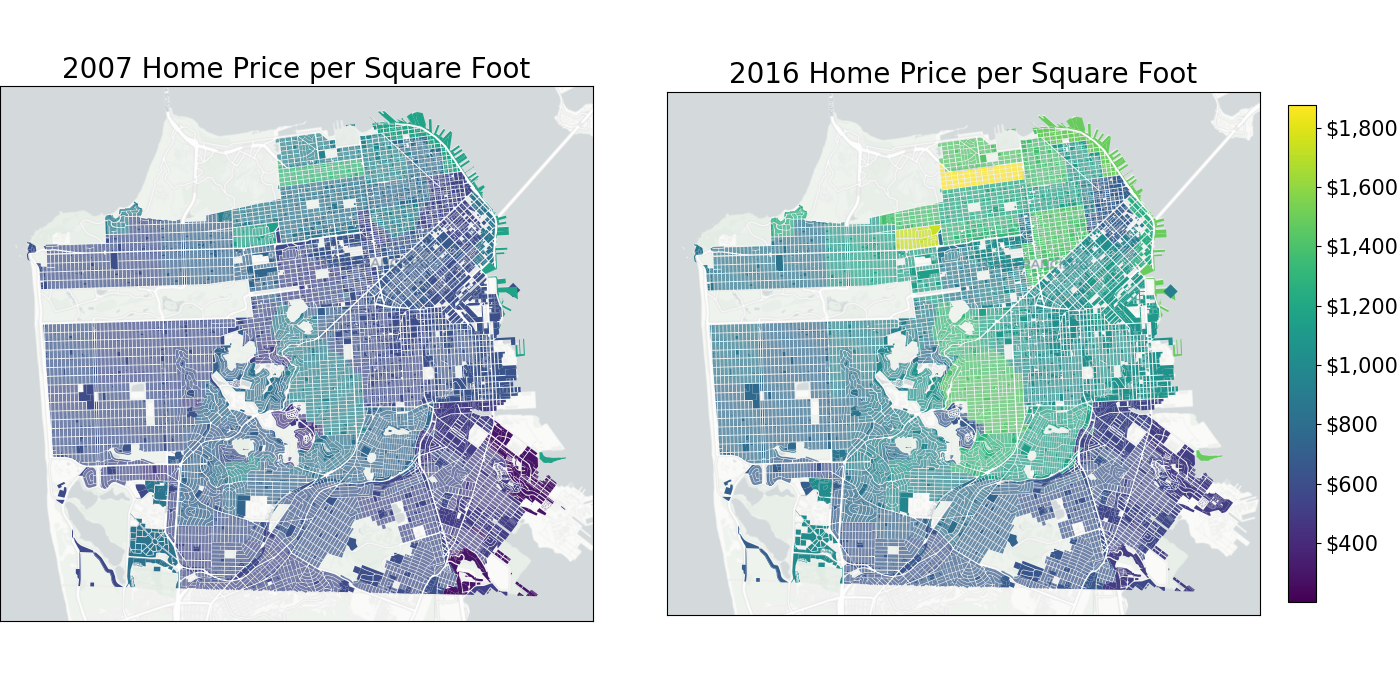
\includegraphics[scale=.45]{figures/combined_sqft_price.png}
    \caption{Home price per square foot is a variable constructed for each parcel in the city at each time step.}
    \label{fig:combined_sqft_price}
\end{figure}

\renewcommand{\arraystretch}{1}

Second, I assume that a parcel, if developed, will be built to the maximum square footage allowed under the city ordinance. (This variable is referred to as the buildable envelope in the SF BlueSky dataset.) 

Third, I assume that residential development projects are sold as condominiums, not rented out as apartments. This is a simplifying assumption that allows me to avoid accounting for discounts for future cashflows because I can assume revenue is made immediately once the condominiums are sold. Furthermore, this resolves a data availability issue because I could not source a dataset that tracked rents at the neighborhood level, but Zillow does provide data on home prices at the neighborhood level.

Revenue itself is a latent variable because there is no extant dataset that tracks the expected revenue of developing housing on given parcels of land. This constructed revenue variable is subject to measurement error.

First, it is not true that parcels, if developed, are built to the maximum square footage allowed under the city ordinance. Often projects are built below the maximum allowed under the city ordinance, but other times projects are built in excess to what the city allows by applying for a variance or by using state density bonus law. Moreover, even if parcels are built to the maximum legal limit, not all square footage can be sold. For example, no revenue is made from building stairwells, elevators, hallways, or a lobby. This is likely a source of measurement error that does not vary by time or location.

Second, the sales price of new units is likely higher than the home values in the neighborhood because there is a premium for new units. However, due to data availability issues, I must make this assumption. It’s not obvious whether this source of measurement error varies by time or location.

Third, \textbf{Table \ref{tab:revenue.pro.forma}} illustrates that the revenue from building homes is actually multi-faceted, but my metric focuses on the most important driver of revenue, which is the residential portion. The revenue gained from retail, in particular, is a trickier source of measurement error because I suspect it is location-dependent and possibly time-dependent. As I understand, the city mandates 25\% of the ground floor be set aside for retail in certain commercial thoroughfares. I include existing commercial uses as a control for this source of measurement error.

\begin{wraptable}{r}{0.5\textwidth}
    \centering
    \caption{Descriptive Statistics for Revenue}
    \label{tab:describe.rev}
    \setlength{\tabcolsep}{10pt}
        \begin{threeparttable}
            \begin{tabular}{rl}
            \hline
            Statistic & Value\tnote{1} \\
            \hline
            Mean & 30.3\\
            Standard Deviation & 206.4 \\
            Minimum & 0 \\
            25\% Quantile & 5.8 \\
            Median & 8.3 \\
            75\% Quantile & 16.5 \\
            Maximum & 26005.3 \\
            \hline
            \end{tabular}
        \begin{tablenotes}
        \item[1]Presented in units of \$100,000.
        \end{tablenotes}
    \end{threeparttable}
\end{wraptable}

Fourth, in \textbf{Table \ref{tab:describe.rev}}, one can see that some parcels are identified as providing zero revenue if built. And yet, these parcels are actually built out somewhat more frequently than parcels identified as yielding slightly greater revenue, per \textbf{Figure \ref{fig:development_vs_revenue}}. The story here is that my revenue metric depends on local zoning ordinances, but developers can request variances to turn low-value non-residential land into higher-value land with the potential for residential use. Because variance requests are riskier, developers tend to go big with their variance requests and request the right to build big buildings, which is why there is a noticeable jump in homes built per parcel for zero-revenue parcels, per \textbf{Figure \ref{fig:production_vs_revenue}}.





\begin{figure}[hbt]
    \centering
    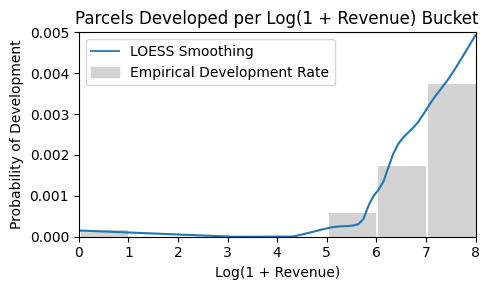
\includegraphics[scale=.75]{figures/development_vs_revenue.png}
    \caption{Probability of development as a function of expected revenue. For visualization purposes, each unit of log(1 + revenue) is treated as a bucket for which the average number of parcels developed is plotted.}
    \label{fig:development_vs_revenue}
\end{figure}


With that caveat aside, \textbf{Figure \ref{fig:development_vs_revenue}} and \textbf{Figure \ref{fig:production_vs_revenue}} illustrate how revenue is otherwise monotonically associated with development outcomes. Parcels with higher projected revenues are more likely to be developed and more likely to be the site of a greater number of homes built. The pearson correlation coefficient with units built per parcel is 0.05, and the pearson correlation coefficient with development is 0.02.\footnote{For the latter correlation, I use the log of revenue, per Figure \ref{fig:development_vs_revenue}.}

\begin{figure}[hbt]
    \centering
    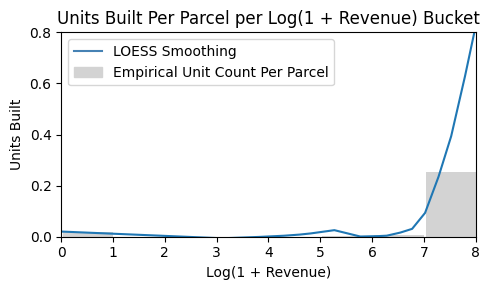
\includegraphics[scale=.75]{figures/production_vs_revenue.png}
    \caption{Units built as a function of expected revenue. Grey bars indicate the average number of homes built among the parcels for each bucketed unit of log(1 + revenue).}
    \label{fig:production_vs_revenue}
\end{figure}

\subsection{Construction Costs}

As indicated in Table \ref{tab:costs.pro.forma}, construction costs are the largest driver of costs of development and can amount to 60\% of total costs. Yet, construction costs are not well understood.\cite{gyourko2006construction} The basic problem is lack of quality data, especially at a high enough resolution to estimate potential construction costs of various developments. Furthermore, housing markets are uniquely localized because homes are built on-site, and so there is great variation in construction costs from one metropolitan area to another.\cite{gyourko2006construction} Typically, policy analysts rely on interviews with developers to get a snapshot of potential construction costs for prototypical projects,\cite{garcia2019making}\cite{la} but this approach does not scale easily.

I overcome this challenge by using a novel approach wherein I frame construction costs as a missing data problem. The non-missing data comes from the San Francisco Department of Building Inspection, which requires developers to state expected costs of construction to get a permit. Using a gradient boosting trees algorithm, I impute expected costs of construction to missing values - viz., to parcels that were not developed in a given year.

With n=1609, I train the gradient boosting algorithm CatBoost, which iteratively builds decision trees as weak learners. The initial algorithm predicts a constant value, and, at each learning iteration, is augmented with a weak learner to minimize an RMSE loss, denoted $L(y,x)$. The algorithm computes the derivatives of the loss for each sample, 

\begin{equation}\label{eq:catboostDerivatives}
\forall i \in \{1,..,n\},   r_{i,m}= -\frac{\partial L(y_{i},f_{m-1}(x_{i}))}{\partial f_{m-1}(x_{i}))}
\end{equation}

where predictor $f_{m-1}$ is a predictor built using $m - 1$ trees. CatBoost then builds a decision tree $t_{m}$ to predict the negative derivatives of the loss using the samples $\{(x_{i},r_{i,m})\}_{x_{i} \in [1,n]}$. The step size towards the direction of gradient descent is controlled by the learning rate hyperparameter $\gamma$. This iterative process is continued until the algorithm either converges or exhausts allotted compute.\cite{prokhorenkova2018catboost} Empirically, a gradient boosting approach achieves excellent results on medium-sized datasets.\cite{bentejac2021comparative}

Another benefit of CatBoost - so-named because it is a boosting algorithm designed for categorical data - is its handling of categorical data, which predominates in my dataset. The conventional approach of one-hot encoding categorical variables poses curse of dimensionality issues for my dataset as some variables, such as one for the property class code, have over a hundred possible values. Rather than one-hot encoding, CatBoost calculates target statistics for categorical values and does so without introducing a prediction shift; specifically, CatBoost randomly permutes the dataset and then computes a target statistic for observation $i$ by calculating the target statistic for $i$ based on its categorical value among observations $j \in \{1, 2, ..., i-1\}$, thereby avoiding a prediction shift.\cite{prokhorenkova2018catboost}

\begin{wraptable}[14]{r}{0.55\textwidth}
    \centering
    \caption{Descriptive Statistics for Imputed Construction Cost Estimates}
    \setlength{\tabcolsep}{12pt}
            \label{tab:impute.construction}

        \begin{threeparttable}
            \begin{tabular}{rl}
            \hline
            Statistic & Value\tnote{1} \\
            \hline
            Mean & 8.9 \\
            Standard Deviation & 48.9 \\
            Minimum & 0.04 \\
            25\% Quantile & 0.8 \\
            Median & 1.3 \\
            75\% Quantile & 2.4 \\
            Maximum & 8000 \\
            \hline
            \end{tabular}
        \begin{tablenotes}
            \item[1]Presented in units of \$100,000.
        \end{tablenotes}
    \end{threeparttable}
\end{wraptable}

Predictions are made on the log scale because doing so ensures the transformation back onto the original scale always yields a nonnegative prediction. Alternative approaches - such as increased regularization or a custom loss function that penalizes negative predictions - failed to eliminate negative predictions on the validation set without reducing model performance. The resulting predictions are presented in \textbf{Table \ref{tab:impute.construction}}: the median project has an estimated \$1,300,000 construction cost, and the mean project construction cost is \$8,900,000, which reflects the right-skewed distribution of housing construction in San Francisco.


I tuned the pipeline with the Python package HyperOpt, a package that performs Bayesian optimization. Unlike random search and grid search, Bayesian optimization learns from past results, making it more compute efficient. I use the expected improvement acquisition function, meaning that each iteration samples the point in the hyperparameter space expected to provide the greatest improvement, which is a function both of the expected value of the response surface at a point as well as the uncertainty around that point of the response surface. \textbf{Table \ref{tab:BoostedCatHyperparameters}} presents results of this Bayesian optimisation with ten iterations of exploration, where each iteration is evaluated based on its mean RMSE across k=5 validation sets in a KFold Cross-Validation setup. The average $R^{2}$ on the validation sets turns out to be greater than 0.73,\footnote{This is from memory. I need to double-check when I get back to statistics computer lab.} implying that most of the variation in unseen data can be explained. 




\begin {table}[tbhp]
\centering
\caption {CatBoost Hyperparameters for Imputing Construction Costs}
\begin{tabular} { @{} p{4cm} p{2cm} p{8cm} @{} }
\toprule
\textbf{Hyperparameters}  & \textbf{Optimal Value} & \textbf{Description}\\
\midrule 
\texttt{boosting\_type} & Plain & The type of boosting used.\\
\texttt{iterations} & 1000 & The total number of trees that are built. \\
\texttt{border\_count} & 101 & The number of splits for numerical features.\\
\texttt{depth} & 7 & The depth of the trees.\\
\texttt{l2\_leaf\_reg} & 0.4071 & Cost function penalty for the L2 norm. \\ 
\texttt{learning\_rate} & 0.0411 & The size of the step taken at each iteration. \\
\texttt{random\_strength} & 0.8843 & The amount of randomness to use for scoring splits when the tree structure is selected. \\
\bottomrule 
\end{tabular}\\
\label{tab:BoostedCatHyperparameters}
\end {table}

The imputed constructions cost estimates turn out to be correlated with the number of homes built, similar to how revenue is correlated with the number of homes built. This makes sense because construction costs are estimated to be higher in parts of the city where the city permits taller buildings like skyscrapers, and these are also the same parts of the city where potential revenue is greatest. I'll return to this after describing the second component of costs.

\subsection{Land Acquisition Costs}

To estimate the cost of acquiring land for each parcel for each year, I relied on tax assessment data. There is, however, a major barrier to relying on the tax assessor's data, which is that the tax assessor is required by law - namely, Proposition 13 - to never increase a tax assessment by more than 2\% per year, unless the property was just sold or rebuilt.

To overcome this, I filter for tax assessments that occur during or immediately after an event that triggers a fair market value reassessment. This yields a dataset of 99,496 observations. As before, I use CatBoost to learn the relationship between parcel attributes and the log of the fair market value assessment of the cost of acquiring the property in a given year. Notably, the fair market acquisition values are extremely right-skewed, and so taking the log of the data ensures that the RMSE loss does not over-emphasize outliers.

Unlike before, I use GroupKFold in this setting because my dataset includes the same parcels at different time steps, and these observations are not independent. Put differently, there's validation set leakage if a model gets to see one time step during training and another time step for the same parcel during validation. Thus, I use GroupKFold where group $i$ is as the set of all time steps $t \in \{1, 2, ... 10\}$ observed for parcel $i$.

Again, I use HyperOpt to tune the hyperparameters for CatBoost, and those results are presented in \textbf{Table \ref{tab:BoostedCatHyperparametersLAC}}. Averaged across k=5 validation sets, the selected model's $R^{2}$ is .958, which is high. 

\begin{table}[hbt]
\centering
\caption{CatBoost Hyperparameters for Imputing Land Acquisition Costs}
\begin{tabular}{@{} p{4cm} p{2cm} p{8cm} @{}}
\toprule
\textbf{Hyperparameters}  & \textbf{Optimal Value} & \textbf{Description}\\
\midrule 
\texttt{boosting\_type} & Plain & The type of boosting to be used. \\
\texttt{border\_count} & 182 & The number of splits for numerical features.\\
\texttt{depth} & 3 & The depth of the trees.\\
\texttt{l2\_leaf\_reg} & 2.52 & Cost function penalty for the L2 norm. \\ 
\texttt{learning\_rate} & 0.303 & The size of the step taken at each iteration. \\
\texttt{subsample} & 0.452 & The fraction of training data used per iteration. \\
\bottomrule 
\end{tabular}\\
\label{tab:BoostedCatHyperparametersLAC}
\end{table}

The second biggest driver of the cost of development is land, per Table \ref{tab:costs.pro.forma}, and accounts for nearly a fifth of the total cost of development. 


   
The imputed values are described in \textbf{Table \ref{tab:ImputedFairMarketAcquisition}}. Manual inspection of the imputed values shows that they are reasonable. For example, the lots that are imputed with a fair market acquisition of a single dollar are actually under water lots or lots that are required by the government to remain vacant, while the most expensive lots to purchase are in the central business district where similarly priced lots are found. The apparently extreme values imputed by CatBoost thus pass a sanity check.

\begin{table}[bth]
    \centering
    \caption{Descriptive Statistics of Imputed Fair Market Acquisition}
    \label{tab:ImputedFairMarketAcquisition}
    \setlength{\tabcolsep}{12pt}
    \begin{threeparttable}
        \begin{tabular}{rl}
        \hline
        Statistic & Value\tnote{1} \\
        \midrule
        Mean & 8.5 \\
        Standard Deviation & 54.6 \\
        Minimum & 0.0 \\
        25\% Quantile & 1.7 \\
        Median & 4.2 \\
        75\% Quantile & 7.8 \\
        Maximum & 8680.2 \\
        \hline
        \end{tabular}
    \begin{tablenotes}
        \item[1]Presented in units of \$100,000.
    \end{tablenotes}
    \end{threeparttable}
\end{table}
   \setlength{\tabcolsep}{0pt}



\subsection{Financial Metric and Measurement Error}
\label{measure.error}

\subsubsection{An Overview to the Financial Metric}
With that, we return to the financial metric $D^*$:
\[
D^* = \frac{R^{*}_{evenue}}{L^{*}_{and} + C^{*}_{onstruction}}
\]
and its corresponding observable $D$:
\[
D = \frac{R_{evenue}}{L_{and} + C_{onstruction}}
\]
where the constructed variable $R_{evenue}$ denotes the revenue gained from selling all units in a housing project, $L_{and}$ denotes the imputed cost of paying to acquire land to build on, and $C_{onstruction}$ denotes the imputed cost of construction. A flowchart recapping how these variables were imputed (or constructed) is provided in \textbf{Figure \ref{fig:flowchart}}.


\begin{figure}[bth]
\caption{Flowchart illustrating that the panel dataset contains all variables that are imputed with CatBoost or constructed, as well as variables contained in the BlueSky dataset of parcels and zoning, the Zillow dataset of home prices, SF DBI's dataset of permits, the tax assessor's dataset, and the topology dataset.}
\label{fig:flowchart}
\centering
\fbox{%
    
    \begin{tikzpicture}[>=Stealth, node distance=1cm]
    
    % Top row
    \node (bluesky) [draw, rectangle, align=center] {bluesky};
    \node (zillow) [draw, rectangle, right=of bluesky] {zillow};
    \node (permits) [draw, rectangle, right=of zillow, shift=1cm] {permits};
    \node (tax) [draw, rectangle, right=of permits] {tax};
    \node (topology) [draw, rectangle, right=of tax, xshift=2cm] {topology};
    
    % Second row
    \node (Revenuedashed) [draw, dashed, rectangle, below=of bluesky, align=left] {construct $R_{evenue}$};
    
    \node (Constructiondashed) [draw, dashed, rectangle, below=of permits, align=left] {impute $C_{onstruction}$};
    \node (Landdashed) [draw, dashed, rectangle, right=of Constructiondashed, align=right] {impute $L_{and}$};
    
    % Penultimate row
    \node (constructD) [draw, dashed, rectangle, below=of Constructiondashed, yshift=-1cm, align=center] {construct $D$};
    
    % Last row
    \node (panelData) [draw, rectangle, below=of topology, yshift=-5cm, align=center] {panel data};
    
    % Arrows and paths
    \draw[->] (zillow) -- (Revenuedashed);
    \draw[->] (bluesky) -- (Revenuedashed);
    \draw[->] (tax) -- (Landdashed);
    \draw[->] (permits) -- (Constructiondashed);
    \draw[->] (tax) -- (Constructiondashed);
    \draw[->] (Landdashed) -- (constructD);
    \draw[->] (Constructiondashed) -- (constructD);
    \draw[->] (Revenuedashed) -- (constructD);
    \draw[->] (constructD) -- (panelData);
    \draw[->] (topology) -- (panelData);
    
    \end{tikzpicture}
}

\medskip
\raggedright
\small{NB: The resulting panel dataset is used in two analyses, each with further data handling required. For the instrumental variable analysis, I merge the panel data with data on accidental fires; for the regression discontinuity analysis, I merge data on impact fees with a 2014 cross-section of the panel data).}
\medskip
\rule{\textwidth}{1pt}
\end{figure}

$D$ is an interaction term between revenue and development costs. The assumption is that revenue and development costs alone do not predict whether housing gets built and that the interaction effect of revenue and development costs matters as well. This assumption is plainly correct, and it should hold true if $D$ measures what it is intended to measure. As a sanity check on $D$, I validate that this interaction term exists in \textbf{Figure \ref{fig:revenue_vs_cost_interact}}. At all terciles for development costs, it is better to project higher revenue, but the effect of increasing revenue is greatly increased when development costs are high. This result is counter-intuitive because it implies that increasing development costs for high-revenue parcels actually increases the average number of units built. This counter-intuitive result is a spurious correlation that stems from the fact that high development costs are a byproduct of being able to build a bigger building. I expect that exogenous shocks to development costs will have the intuitive result - viz., lower development costs improve the outlook for homebuilding.

\begin{figure}[hbt]
    \centering
    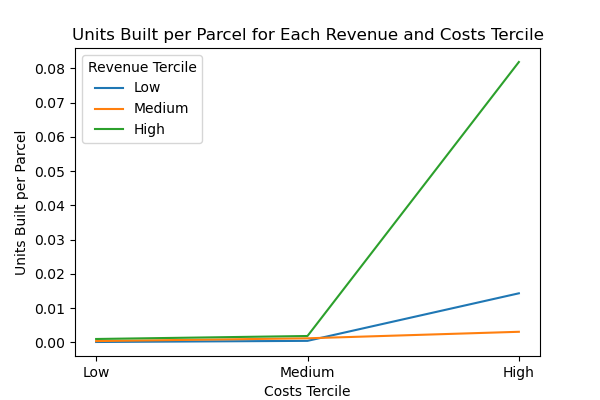
\includegraphics[scale=.75]{iv/revenue_vs_cost_interact.png}
    \caption{Evidence of two-way interaction effect between revenue and cost on units built.}
    \label{fig:revenue_vs_cost_interact}
\end{figure}



This spurious correlation also implies that $D$ does not have the intuitive univariate relationship with development rates. As indicated in \textbf{Figure \ref{fig:d_vs_proportion_developed}}, there is no monotonically increasing development rate as a function of $D$. Thus, while the interaction between revenue and costs clearly exists, $D$ does not capture this interaction the way other financial metrics do. (Or, at least, the effect of $D$ is not clear without first controlling for R and C.)

\begin{figure}[hbt]
    \centering
    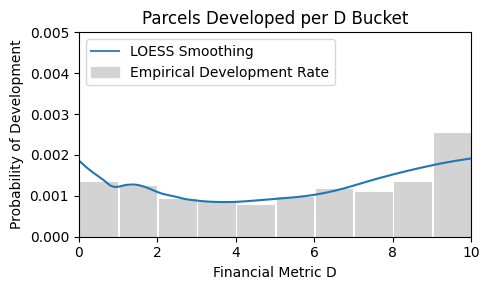
\includegraphics[scale=.75]{figures/development_vs_D.png}
    \caption{Relationship between rate of housing development and financial metric $D$.}
    \label{fig:d_vs_proportion_developed}
\end{figure}


\subsubsection{Measurement Error}

There are two sources of measurement error: first, there is multiplicative measurement error associated with the latent variables; second, there is noise from imputation. I'll take these in turn. 

First, to simplify the problem of estimating $D^*$, I assume that the error in measuring $R^*$, $L^*$, and $C^*$ are multiplicative so that I can take the log of $D*$ and get asymptotically consistent estimates of its effect. 

As argued in Section \ref{rev.sec}, it is reasonable that
\[
R^{*}_{evenue} = \gamma_0  \gamma_{zt} R_{evenue}  
\]
where $\gamma_0$ is a
source of measurement error that does not vary by time or location (like the premium paid for new construction as compared to existing units, or the portion of built space that can be sold for residential use), and $\gamma_{zt}$ is a source of measurement error that varies according to the zoning and time step of an observation. These sources of error are multiplicative because they affect both the effective rent charged per square foot built and also the square foot built. To make this tractable, I assume the location-dependent measurement error is not at a parcel-level (which would be unrealistic in any case) and instead assume this latter measurement associated with $\gamma_{zt}$ depends on the parcel's zoning $z$ and time step $t$. Zones of the city are regulated disparately by the city over time, and this mismeasurement could stem from how these policies change over time. In particular, I have in mind the measurement error that stems from changes in where the city mandated retail space be included in residential projects; while there is no dataset of such policy changes over time, controlling for $log(\gamma_{zt})$ is sufficient.

Likewise, I assume $L^* = \phi L$ and $C^* = \delta C$ where $\delta$, $\phi \in \mathbb{R}$. For $L^*$, this multiplicative error could potentially capture systematic undervaluation of parcels' value by the tax assessor. For $C^*$, this multiplicative error could capture systematic undervaluation of the construction costs of projects. (There is even evidence in the SF DBI dataset that developers typically underestimate their project costs and revise them upwards at later dates.) 

Putting this together, the latent financial metric $D^*$ reduces to:

\begin{align*}
D^* &= \frac{R^*}{L^* + C^*} \\
 &= \frac{R \tilde{\gamma_{zt}}}{L \phi + C \delta}
\end{align*}

where $\tilde{\gamma_{zt}}$ = $\gamma_{0}\gamma_{zt}$. And by taking the log of both sides, 

\begin{align*}
log(D^*) &= log(R) + log(\tilde{\gamma_{zt}}) - log({L \phi + C \delta}) \\
 &= log(R) + log(\tilde{\gamma_{zt}}) - log(L + C) - log(\delta) \\
  &= log(D) + log(\tilde{\gamma_{zt}}) - log(\delta)
\end{align*}

where the second inference requires the assumption that $\delta = \phi$. Testing this assumption empirically with proxies is feasible, but difficult to accomplish in the scope of this dissertation. While the SF DBI dataset has evidence on the rate of undervaluation of construction projects, it is hard to come by non-proprietary datasets of large real estate transactions with which we could compare the systematic undervaluation of property of the tax assessor.\footnote{Furthermore, future work could use empirical estimates of proxies, like those just mentioned, for $\delta$ and $\phi$, and thereby find a correction factor.}

The measurement error attributable to $log(\delta)$ will be subsumed by the intercept term, and the measurement error attributable to $log(\tilde{\gamma_{zt}})$ will be accounted for in an intercept for the interaction of zoning and the time step. While those coefficients would no longer have their standard interpretations, the measurement error would not get subsumed by the error term $u_{it}$, so the estimate for $\beta_{D}$, the partial effect of D, would remain consistent.

To make this argument, however, I must exclude parcels with an estimated revenue of zero dollars, which accounts for 0.8\% of observations, and for which $D$ is zero. These parcels are parcels where it is illegal to develop anything. The log of zero is undefined, and the standard workaround of adding a positive constant is incompatible with the multiplicative error argument. Like other policy analyses of the supply effects of housing legislation, my analysis excludes parcels that are not currently developable under law.

Turning to the second source of measurement error, let's consider the noise induced by the imputation method. There's inherent uncertainty in the values imputed by CatBoost, as evidenced by the fact that different random seeds will yield different predictions. This uncertainty would not be reflected in the standard errors reflected by OLS fit to $D$. Assume the measurement error attributable to imputation is as follows:
\begin{align*}
log(D) = log(\tilde{D}) + \epsilon_{D}
\end{align*}

where $log(\tilde{D})$ is the unobserved variable and $\mathbb{E}[\epsilon_{D}]=0$, and Cov$(log(\tilde{D}), \epsilon_{D}) = 0$. By consequence, Cov$(log({D}), \epsilon_{D}) \neq 0$. This is the classical errors-in-variables assumption, for which attenuation bias becomes a concern.\cite{wooldridge2010econometric} That is, one would expect the absolute value of the $\hat{\beta_{D}}$ estimate to be shrunk towards zero, and all the estimate coefficients in an OLS regression would be inconsistent.\cite{wooldridge2010econometric} 

Per Wooldridge, the variance of the measurement error is equal to the covariance between the observed $log(D)$ and the measurement error:\cite{wooldridge2010econometric}
\[
\text{Cov}(log(D), \epsilon_{D}) = \mathbb{E}[log(D)\epsilon_{D}] = \mathbb{E}[log(\tilde{D})\epsilon_{D}] + \mathbb{E}[\epsilon^2_{D}] = \sigma^2_{\epsilon_{D}}
\]

This motivates using an algorithm like CatBoost for the imputation strategy. By picking hyperparameters to minimize the RMSE on unseen data, my imputation strategy is effectively minimizing the variance of the noise term, $\sigma^2_{\epsilon_{D}}$, which can be estimated via the variance of residuals on a validation set. As a result, excellent generalization to new unseen data is mitigating this source of measurement error. Empirically, gradient boosting algorithms like CatBoost achieves excellent results in generalizing.\cite{bentejac2021comparative} Moreover, CatBoost in particular, as compared with other gradient boosted algorithms, reduces noise associated with the curse of dimensionality, as CatBoost calculates target statistics which obviate the need for one-hot encoding categorical variables. For the dataset at hand, one-hot encoding would create hundreds of additional dimensions that would increase the noise of my estimates, and thereby increase $\sigma^2_{\epsilon_{D}}$. 

Furthermore, and crucially, my motivation for employing an instrumental variable analysis is to mitigate the remaining measurement error because, for the instrument $Z$, it is reasonable that Cov$(Z, \epsilon_{D}) = 0$, and so conditioning for $Z$ purges the measurement error from $log(D)$.

As future work, one could incorporate Multiple Imputation by Chained Equations (MICE) to update the standard errors reported to account for uncertainty from imputations. MICE creates multiple imputed datasets and pools together analysis conducted on each dataset, which means it is possible to quantify the uncertainty created as a result of missing data. Where imputations are less certain as evidenced by variability in the values imputed, the standard errors would increase in the pooled analysis.\cite{azur2011multiple} In the absence of this approach, I simply run a robustness check by rerunning the imputations a second time with different random seeds to ensure the magnitude of the error is negligible on the estimated coefficient.\footnote{See the iv\_analysis.Rmd file in the github repository for the outputs of this analysis.}

\section{Exploratory Data Analysis}

\subsection{Building housing is rare}

In all, there are 1,838 cases where housing is built in a panel dataset of N=1,531,273. Thus, zeros dominate the dataset and account for 99.87\% of all observations. A zero-inflated dataset is what we would intuitively expect, as buildings typically last sixty years before being torn down. But San Francisco's regulatory environment, in particular, makes it difficult to build new housing, as evidenced by the map (see \textbf{Figure \ref{fig:age}}) of the average age of residential buildings.

When housing is built, most housing projects add just one or two homes, but a few housing projects make up the bulk of what the city builds, as indicated by \textbf{Table \ref{tab:NetUnitsCompleted}}. The two largest projects (with 500+ units each) alone account for more units built than the 1177 single-unit projects.


\begin{table}[hbt]
\centering
\caption{Number of Observations for Different Buckets of Residential Project Size}
\setlength{\tabcolsep}{10pt} 
\begin{tabular}{r|cccccccccccc}

\hline
\textbf{Units Built} & 1 & 2 & 3 & 4 & 5-10 & 11-199 & 200-399 & 400+ \\
\hline
\textbf{Count} & 1177 & 235 & 83 & 48 & 58 & 131 & 11 & 11 \\
\hline
\end{tabular}
\label{tab:NetUnitsCompleted}
\end{table}



\subsection{Spatial and temporal trends in homebuilding}
Development trends vary greatly by year, as interest rates, labor availability, and raw material expenses like wood vary greatly year to year. In particular, as shown in \textbf{Figure \ref{fig:eda_year_trend}}, a downturn in housing construction coincides with the Great Recession of 2008.

Development trends also vary spatially. Pooling together all years of the panel dataset, \textbf{Figure \ref{fig:eda_spatial_trend}} shows where housing gets built. Each red circle reflects a housing development, with the size indicating how many units of housing were built as part of the development: large circles reflect large apartment (or condo) complexes. As can be seen, most of the total units built are built on the east side of the city. The west side of the city, in comparison, sees development, but of a very different type: namely, backyard homes, also known as in-law units.

\begin{wrapfigure}[12]{r}{0.6\textwidth}
    \centering
    \caption{Units built per year.}
    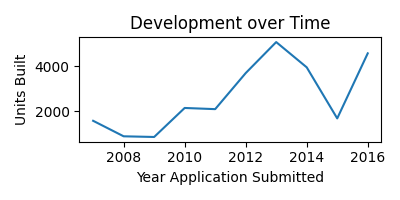
\includegraphics[scale=.9]{figures/development_over_time.png}
    \label{fig:eda_year_trend}
\end{wrapfigure}







\begin{figure}[hbtp]
    \centering
    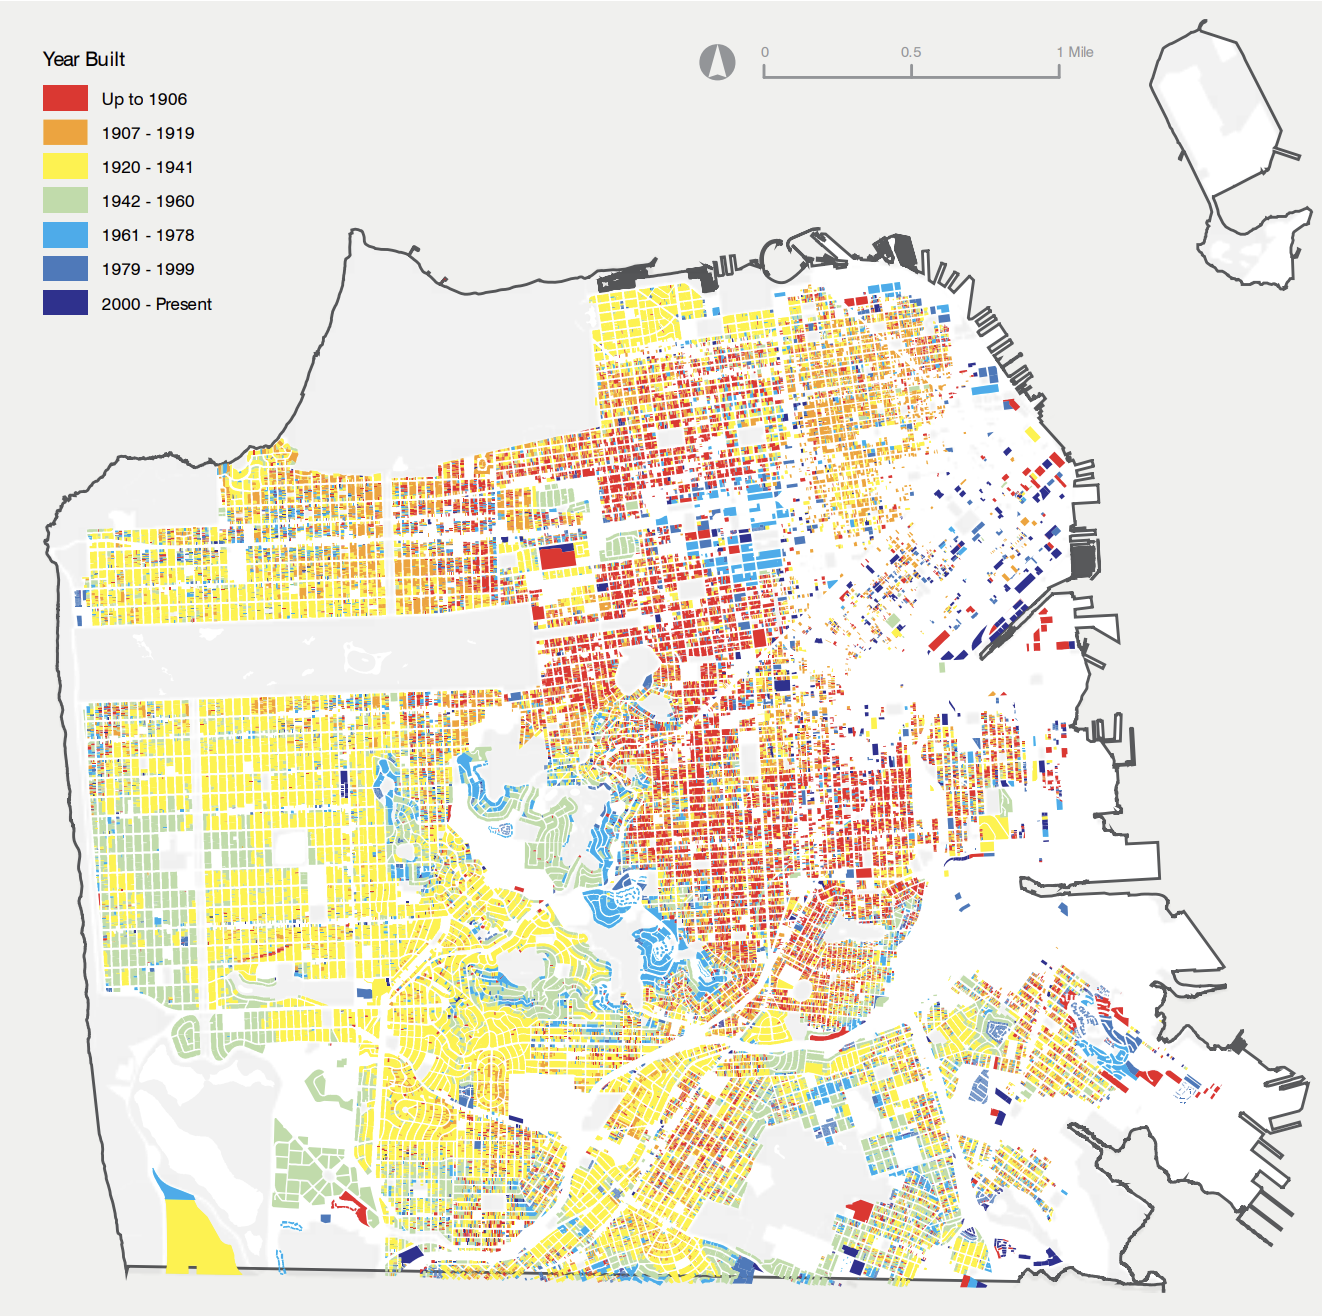
\includegraphics[scale=.6]{figures/age.png}
    \caption{All Housing by Year Built. Figure 29 of SF Constraints Report.\cite{SFHousingElement2022}}
    \label{fig:age}
\end{figure}

\begin{figure}[hbt]
    \centering
    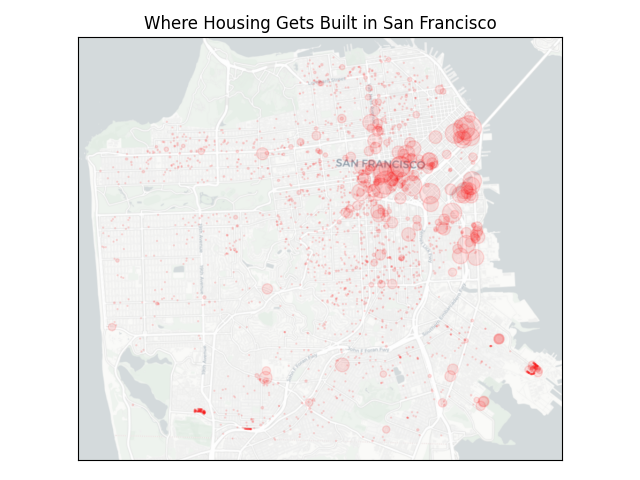
\includegraphics[scale=.85]{figures/where_housing_gets_built.png}
    \caption{Spatial trends in homebuilding. Marker size reflects \# of units built at location.}
    \label{fig:eda_spatial_trend}
\end{figure}

As a result, it is worth considering fixed effects for time and neighborhood.

\subsection{Other predictors of homebuilding}
In \textbf{Figure \ref{fig:eda_barplots}}, there is evidence that properties with existing residential uses - especially single family residence - are less likely to be redeveloped into housing. This confirms the intuition outlined in Section \ref{data.sources} that San Francisco's anti-demolition ordinances to protect tenants reduce housing production, as intended. Furthermore, it's striking that parcels with an existing use that's categorized as Miscellaneous/Mixed-Use are much more likely to be developed into housing, at roughly three times the rate of other parcels.

\begin{figure}[hbt]
    \centering
    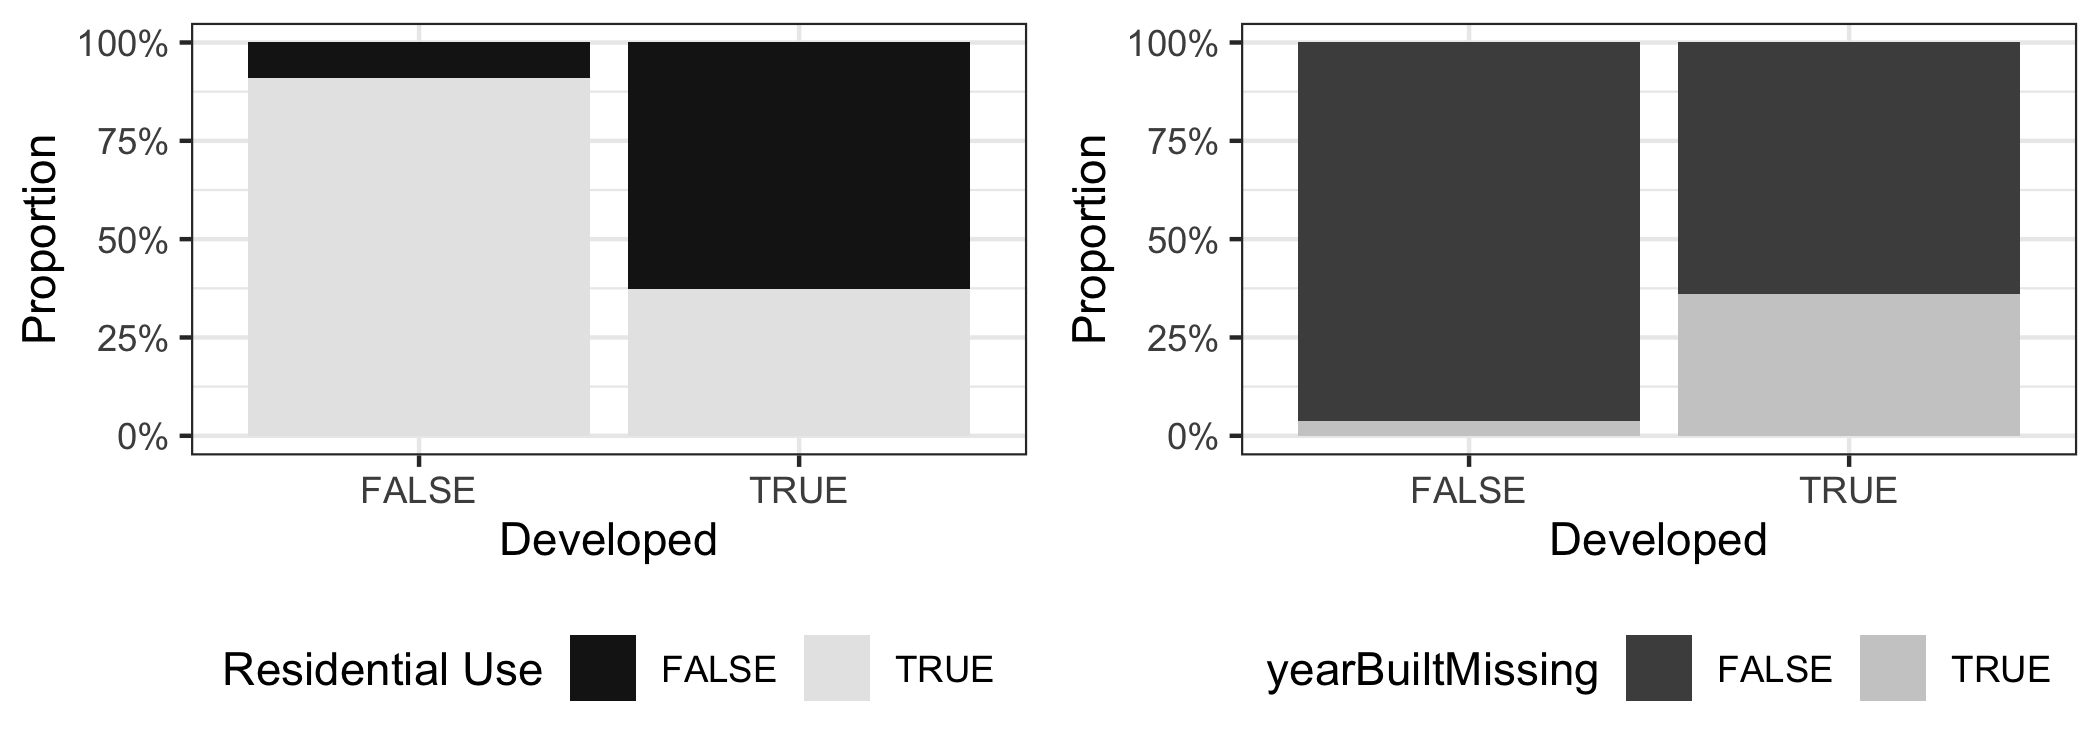
\includegraphics[scale=.85]{pdev/figures/eda_barplots.png}
    \caption{Development rates of parcels based on the existing use.}
    \label{fig:eda_barplots}
\end{figure}


In \textbf{Figure \ref{fig:eda_boxplots}}, one can see strong evidence that properties where zoning permits a large increase in square footage are much more likely to be redeveloped into housing. This is intuitively obvious as the profit of development has much to do with the amount of additional rent that can be charged, which goes hand in hand with the amount of new square footage for which rent can be charged.

\begin{figure}[hbt]
    \centering
    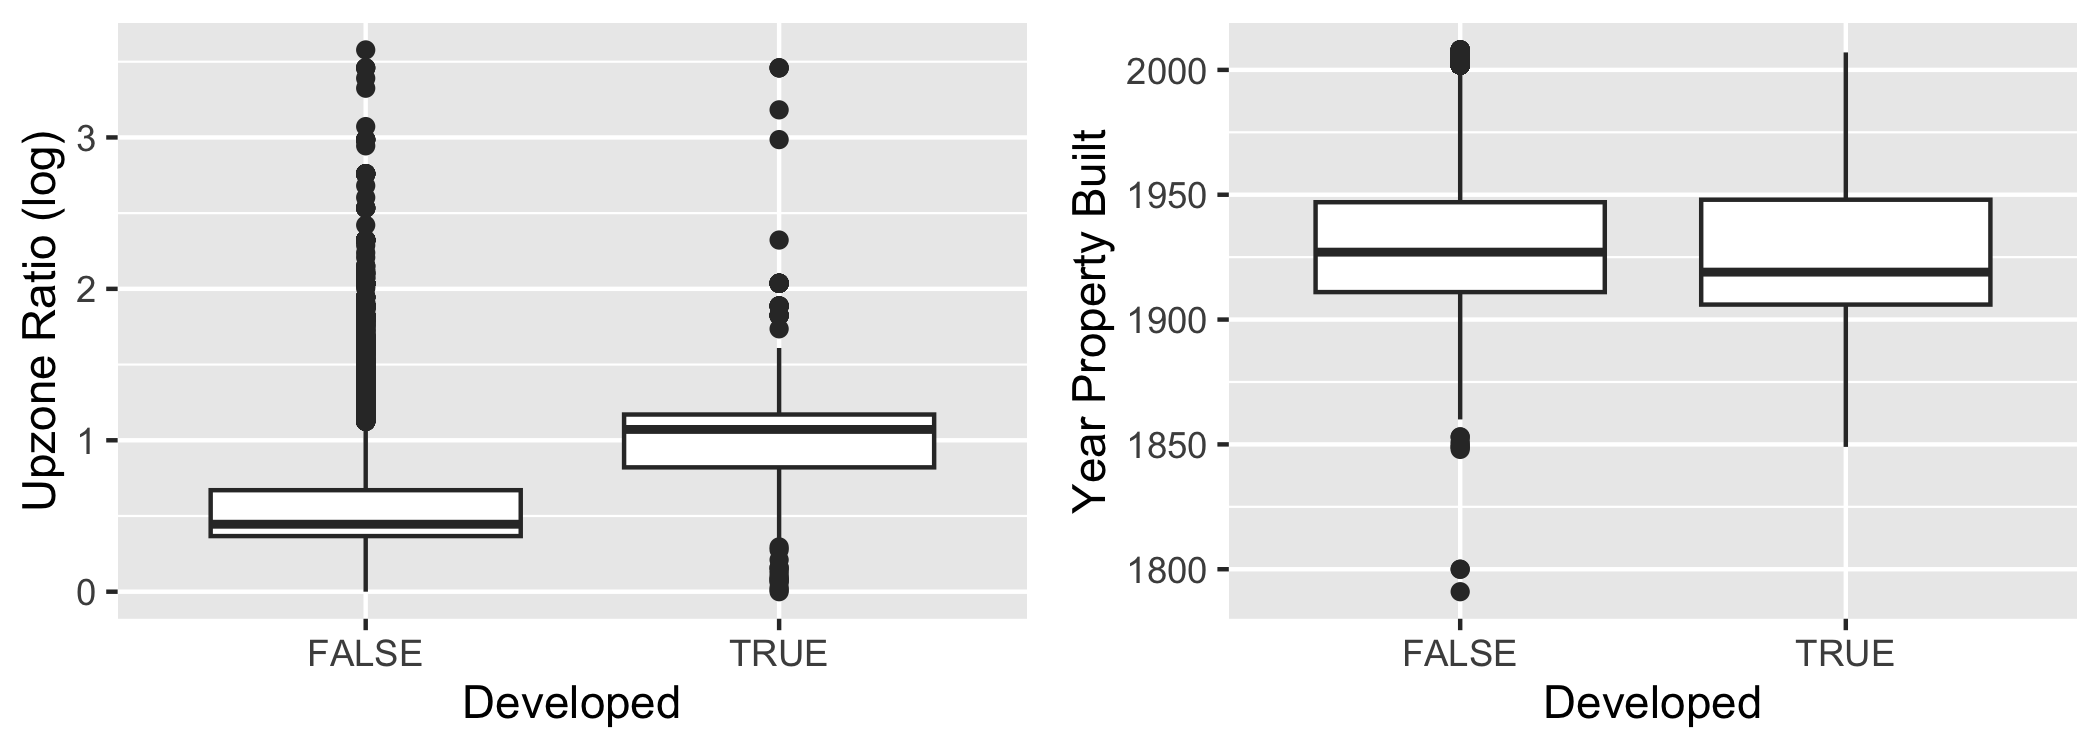
\includegraphics[scale=.8]{pdev/figures/eda_boxplots.png}
    \caption{Log of upzone ratio (left) is moderately related to whether parcels are developed or not. Parcels sold recently are much more likely to be redeveloped (right).}
    \label{fig:eda_boxplots}
\end{figure}

Per \textbf{Table \ref{tab:correlation_with_developed}}, most variables are weakly correlated with whether or not housing is built. The variables displayed are those with the largest absolute value r, and so most variables have virtually no correlation at all with whether housing is developed. A priori, however, one should not expect strong linear, univariate relationships between these variables and development for the simple reason that development is mediated by financial metric analyses that involve the non-linear interaction of half a dozen variables, including rent, land values, zoning, and various neighborhood-level factors like impact fees. One simple example of such interaction effects is included in \textbf{Figure \ref{fig:two_way_res_history}}, which illustrates that there is a two-way interaction effect between an existing residential use and historic resource status. The fact that the confidence intervals are non-overlapping and that the slopes intersects implies the existence of a two-way interaction effect. I provide this figure not to single out these two particular variables, but merely to illustrate the general point that these interaction effects abound because financial metrics themselves are the interaction of many factors.





\begin{table}[hbt]
\centering
\caption{Pearson Correlation Coefficients with Binary Indicator for Development}
\setlength{\tabcolsep}{10pt} 
\begin{tabular}{r l}
\hline
\textbf{Variable} & \textbf{Correlation with Development} \\
\hline
Years Since Last Sale & -0.032 \\
Imputed Construction Cost& 0.030 \\
Upzone Ratio  & 0.025 \\
Federal Reserve Interest Rate  & 0.019 \\
Existing Residential Use & -0.019 \\
Citywide Home Price & 0.019 \\
Homeowner Exemption Value & -0.019 \\
Year & 0.018 \\
Form-Based Zoning & 0.018 \\
Local Home Price Per Sq Ft & 0.016 \\
\hline
\end{tabular}
\label{tab:correlation_with_developed}
\end{table}

\begin{figure}[hbt]
    \centering
    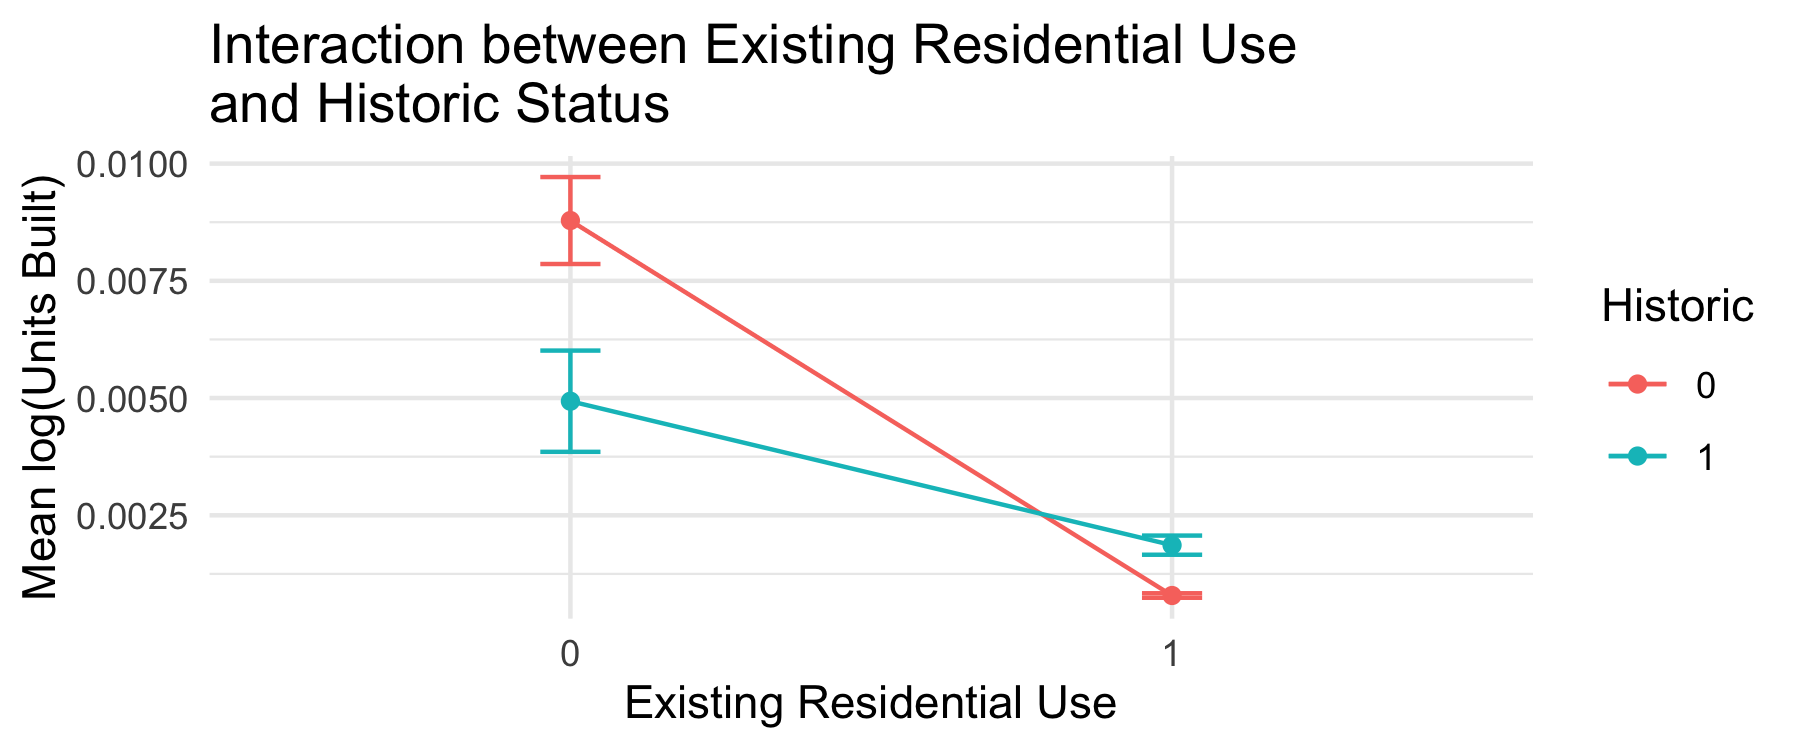
\includegraphics[scale=.2]{figures/two_way_res_history.png}
    \caption{Comparing Mean of log(Units Built) for parcels, disaggregated by existing residential use and historic status, with 90\% Confidence Intervals.}
    \label{fig:two_way_res_history}
\end{figure}


\begin{table}[ht]
\centering
\setlength{\tabcolsep}{10pt} 
\caption{Pearson Correlation Coefficients with Count of Homes Built on Parcel, Conditioned on Housing Being Developed}
\begin{tabular}{r l}
\hline
\textbf{Variable} & \textbf{Correlation with \# of Homes Built} \\
\hline
          Imputed Development Costs & 0.718 \\
          Imputed Construction Cost & 0.702 \\
          Imputed Revenue & 0.597 \\
          Buildable Envelope  & 0.540 \\
          Upzone Ratio  & 0.537 \\
          Office/Commercial Zone     &  0.373   \\
          Existing Residential Use &  -0.373  \\
           Imputed Land Acquisition Cost &  0.352 \\
            Property Area  & 0.322   \\
           Assessed Land Value         &  0.318  \\
\hline
\end{tabular}
\label{tab:correlation_with_count_homes}
\end{table}



Given that housing is built, a slightly different set of factors are relevant to how much housing is built, as outlined in \textbf{Table \ref{tab:correlation_with_count_homes}}. (Note that only the ten variables with the largest absolute value correlation are shown.) For example, the land values and the area of the land have a more significant role. Additionally, the estimated construction costs are highly predictive of how many homes will be built, which intuitively makes sense as the higher construction costs are reflective of the fact that more homes are anticipated to be built.

\section{Analysis}
\label{analysis.sec}
As argued at the end of Section \ref{exist.policy.analysis}, the treatment $D$ is endogenous to housing production. Parcels that are financially viable to build housing on are, to a large extent, financially viable because the city regulates them favorably.\cite{monkkonen2016understanding} That decision itself reflects other factors like the stance of local interest groups, the weighing of trade-offs involving historic resources, and so on.\cite{dougherty2020golden} These other factors have clear causal impacts on housing production that are not mediated solely through $D$. For example, the opposition of local homeowner groups both affects D through housing policy and also directly affects housing production insofar as local homeowners resistant to change are less interested in developing their own parcels.

Formally, a regression-based test derived by Hausman can verify that D is endogenous to housing production.\cite{wooldridge2010econometric} First, using OLS, I regress D as a function of exogenous variables in a two-way fixed effects model; then I regress log(homes built) on the exogenous variables and the residuals of the first model. Using sandwich estimators for standard errors, I find the residuals are statistically significant far below the $\alpha=0.01$ level across all sandwich estimators used (see \textbf{Table \ref{hausman.endog.test}}). Thus, D is endogenous, and so an OLS estimate of D's partial effect is inconsistent.\footnote{Notably, this test is asymptotically equivalent to the test of whether the Two-Stage Least Squares (2SLS) and the OLS estimates of the partial effect of $D$ are equivalent.\cite{wooldridge2010econometric}}
\setlength{\tabcolsep}{10pt} 

\begin{table}[bth]
    \centering
    \caption{Robust Tests for Endogeneity of $D$}
    \begin{tabular}{|c|c|c|c|}
        \hline
        Method & Weighting & p-value & 95\% Confidence Interval \\
        \hline
        white1 & HC1 & 0.0029 & [-0.0011, -0.0002] \\
        white1 & HC3 & 0.0030 & [-0.0011, -0.0002] \\
        arellano & HC1 & 0.0012 & [-0.0011, -0.0003] \\
        arellano & HC3 & 0.0013 & [-0.0011, -0.0003] \\
        \hline
    \end{tabular}
    \label{hausman.endog.test} \\
    \raggedright
    \medskip
    \small{Multiple robust sandwich estimators are presented to demonstrate robustness to assumptions. Arellano's method permits serial, cross-sectional correlation, while both methods permit general heteroscedasticity.}
    \bottomrule
\end{table}

To address this endogeneity, I provide an instrumental variable (IV) estimate of the partial effect of $D$. In addition to providing an IV estimate, I also provide a regression discontinuity analysis of the average treatment effect (ATE) of $F$, a binary treatment where neighborhood-specific impact fees - where are fees levied per square foot of residential construction - are increased by 50\%. While these are separate quantities to estimate, and while the ultimate goal is to estimate the partial effect of $D$, I provide these two methods in aspirations that they provide similar estimates. In particular, I can evaluate what the estimated partial effect of $D$ would be for a decrease in the dollar amount equivalent to the fee reduction $F$ and evaluate how close that point estimate is with the point estimate for the average treatment effect (ATE) of $F$.

Relying on an RDD to estimate the effect of F also has the added benefit that it can provide a robustness check on the mismeasurement of $D$, in addition to the typical robustness check to the methodological decisions made in the IV analysis.


\begin{figure}[hbt]
    \centering
    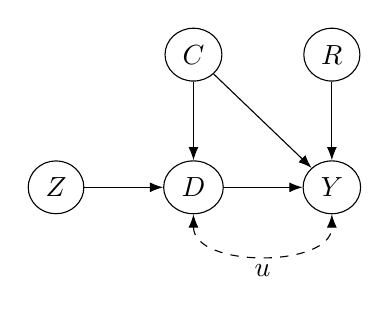
\begin{tikzpicture}
        \node[state] (1) {$Z$};
        \node[state] (2) [right =of 1]  {$D$};
        \node[state] (3) [right =of 2] {$Y$};
       \node[state] (5) [above =of 2] {$C$};
        \node[state] (6) [above =of 3] {$R$};
        \path (1) edge node[above] {} (2);
        \path (2) edge node[above] {} (3);
        \path (5) edge node[right] {} (2);
        \path (5) edge node[right] {} (3);
        \path (6) edge node[right] {} (3);
        \path[bidirected] (2) edge[bend right=90] node[below] {$u$} (3);

    \end{tikzpicture}
    \caption{A structural causal model of financial metric $D$ affects housing development. }
    \label{fig:scm1}
\end{figure}

Above, Z is an instrumental variable, namely accidental fires; $D$ is the observable measure of financial metric $D^*$; C is the set of observed confounders that are unaffected by the instrument; R is the set of variables that explains housing production unrelated to $D$; Y is the housing produced in a given year on a given parcel.

A few words are in order to explain how my data fits into the structural causal model illustrated in \textbf{Figure \ref{fig:scm1}}. In my dataset, every covariate aside from the instrument plausibly has a direct causal effect on Y, as I sketched out in Section \ref{data.sources}. 

Certain variables, R, causally affect Y and not indirectly through the treatment. For example, I use DBI's permits dataset to track which parcels recently pulled a permit to make an improvement to the existing structure on the land. This surely affects the likelihood of development on the parcel because a recent improvement is indicative that the owner is interested in maintaining the site's existing use.  (Note that nothing in my analysis hinges on these variables R \textit{not} being a confounder. If they happen to be confounders, then I control for them all the same.) I control for variables R to improve the precision of my estimate.\cite{cinelli2021crash}

Notably, all but one of my covariates that I control for are pre-treatment covariates, so they cannot be causally determined by the treatment D. The one exception is the 2019 topological data, which is post-treatment, but assuredly is not downstream of any causal chain set off by the treatment. Hence, I avoid introducing bias by controlling for a mediator.\cite{cinelli2021crash}

% There is a subtle issue in whether to control for variables that are inputs to the financial metric D. On one hand, they may appear to be confounders if they also have a direct effect on Y. However, I choose not to control for these variables unless they plausibly have a direct effect that is not mediated by D*. Otherwise, because D is a function of D*, controlling for such variables is actually controlling for an instrument of D, which reduces precision.

\subsection{Instrumental Variable}

\subsubsection{Method}

My population model is as follows:
\[
log(1 + Y_{it}) = \alpha_0 + \beta_{D}log(D_{it}) + x_{zt} + \mu_{i} + \theta_{t} + u_{it}
\]
where $i$ indexes the parcel, $t$ indexes the year, $z$ indexes the zone, $x_{zt}$ is an intercept for two-way interactions between the zoning and the year, $\mu_{i}$ are parcel-level effects that do not vary over time, $\theta_{t}$ is an intercept for each time step, $\alpha_{0}$ is an intercept, and $u_{it}$ is a disturbance with $\mathbb{E}[u_{it}] = 0$. The estimate of interest is the partial effect of $log(D^*_{it})$ on the conditional expectation of $log(1 + Y_{it})$.

I estimate this using 2SLS with a two-way fixed-effects panel model, with the first stage defined as follows:
\[
log(D_{it}) = \alpha_{0} + \lambda Z_{it} + \mu_{i} + x_{zt} + \theta_t + \epsilon_{it}
\]
where $Z_{it}$ is an instrumental variable and $\epsilon_{it}$ is an error term with expectation zero; and the second stage defined as follows:
\[
log(1 + Y_{it}) = \alpha_0 + \beta_D \hat{log(D)}_{it} + \mu_i + x_{zt} + \theta_t + u_{it} 
\]
where $\hat{log(D)}_{it}$ is the fitted value from the first stage.

The desiderata for the instrumental variable $Z$ are threefold: first, $Z$ must be relevant and causally affect the treatment $D$; second, $Z$ must satisfy the exclusion-restriction requirement that its total effect on the outcome be mediated by the treatment; and third, $Z$ must be exogenous, meaning that $Z$ cannot be confounded by an observed or unobserved variables. I will take up these considerations in turn in Section \ref{fires.instrumnet}.

\subsubsection{Accidental Fires as an Instrument}
\label{fires.instrumnet}
Previous research has already used accidental fires as an instrumental variable and found that serious, accidental fires strongly predicted housing production.\cite{pennington2021does} Accidental fires are correlated with development, as indicated in \textbf{Table \ref{table:fire_vs_development_punnett}}, which displays the parcels which by time step $t$ had a fire and whether it had development at time step $t$.  Per \textbf{Figure \ref{fig:fires.dev}}, fires are associated with a 7.14x increase in development rate.

\begin{table}[hbt]
    \centering
    \caption{Exposure to Accidental Fire Versus Development Outcomes}
    \setlength{\tabcolsep}{10pt} 
    \label{table:fire_vs_development_punnett}
    \begin{tabular}{lcc}
        \hline
         & No Development & Had Development \\
        \hline
        No Fire & 1527254 & 1820 \\
        Had Fire & 1709 & 11 \\
        \hline
    \end{tabular}
\end{table}

\begin{figure}[hbt]
    \centering
    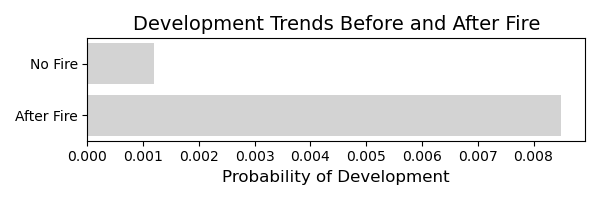
\includegraphics[scale=.8]{iv/dev_fire_fstat.png}
    \caption{Development trends with and without fire.}
    \label{fig:fires.dev}
\end{figure}

In all, there are 302 unique accidental fires that are serious enough to cause damage to the building in my dataset. As indicated in \textbf{Table \ref{table:fire_vs_development_punnett}}, serious accidental fires are relatively rare events, as is development. In total, only eleven parcels both were the site of a fire and had development, meaning that my analysis hangs on a small number of highly influential plots.

The story for why this effect would be mediated through the financial metric $D$ is as follows: if an accidental fire diminishes property values, then that reduces land acquisition costs, increasing the economic return of developing a project on that parcel of land. A priori, the case for the relevance of this candidate is clear.

In fact, it is trivial that the instrument and exposure are correlated because the treatment is constructed as a function of the instrument. In particular, in San Francisco Fire Department logs, fire fighters record the estimated property damage caused by a fire. Notably, they disaggregate damage to the building from damage to personal belongings. This is important because real estate transactions don't typically include personal belongings, so I can isolate the damage caused by the fire that actually lowers the cost of the property sale. I then subtract this estimate from the land acquisition costs in my formula for $D$. Where the fire department's estimated property damage exceeds the fair market value of the property built on top of the land, I clip the value so it is never negative.

Validating the relevance, the partial F-statistic is 1729.3 and the p-value is vanishingly small. Typically, a threshold of 10 is suggested for the partial F-statistic. The partial r-squared, however, is very small at 0.001.

I considered using the dollar amount of the fire damage as the instrument since that value has a large impact on $D$. However, when testing whether the instrument was independent of observed confounders, I regressed log(fire damage) on key potential confounders, like whether the existing use is residential, whether the lot is zoned for office development, how much square footage one is allowed to build (envelope 1000), and how that compares with the size of what's currently built (upzone ratio). Per \textbf{Table \ref{table:fire.o.c.regression_output}}, log(fire damage) is significantly correlated with the four observed confounders I tested. The standard errors presented in Table \ref{table:fire.o.c.regression_output} are robust for heteroscedasticity.


\begin{table}[hbt]
    \caption{Testing whether the continuous instrument of log(fire damage) is notable independent of observed confounders}
    \label{table:fire.o.c.regression_output}
    \setlength{\tabcolsep}{10pt} 
    \centering
    \begin{tabular}{lcccc}
        \hline
        Term & Estimate & Std. Error & t value & Pr(>|t|) \\
        \hline
        Upzone Ratio & 0.00 & 0.00 & 2.87 & 0.0041 \\
        Buildable Envelope & 0.00 & 0.00 & 10.39 & < 2.2e-16 \\
        Existing Residential Use & -0.01 & 0.00 & -5.91 & 3.36e-09 \\
        Office/Commercial Zone & 0.02 & 0.00 & 3.38 & 0.0007 \\
        \hline
    \end{tabular}
\end{table}


This suggests that fires that cause a lot of damage, inherently, burn down big buildings, which means that something big \textit{can} be built on that parcel under the city's zoning ordinance. This would then be correlated with other confounders that are related to zoning.

As a result, my instrument is the binary variable indicating whether a fire took place or not, rather than a continuous variable indicating the log of the damage caused by the fire. This is mostly successful, as evidenced by the updated p-values in the logistic regression output in \textbf{Table \ref{table:fire.binom.o.c.regression_output}}.

\begin{table}[hbt]

    \caption{Testing whether binary instrument of fire is independent of notable observed confounders}
    \setlength{\tabcolsep}{10pt} 
    \label{table:fire.binom.o.c.regression_output}
       \centering 
    \begin{tabular}{lcccc}
        \hline
        Term & Estimate & Std. Error & z value & Pr(>|z|) \\
        \hline
        Upzone Ratio & -0.018 & 0.059 & -0.30 & 0.761 \\
        Buildable Envelope & 0.0015 & 0.00082 & 1.82 & 0.069 \\
        Existing Residential Use & -0.092 & 0.20 & -0.46 & 0.646 \\
        Office/Commercial Zone & 0.47 & 0.32 & 1.48 & 0.138 \\
        \hline
    \end{tabular}
\end{table}

The exclusion-restriction assumption is arguably tenuous. It is plausible that some accidental fires may have a direct effect on housing production not mediated by economic feasibility if the fire burned down a home that the previous residents want to rebuild and return to, economic costs notwithstanding. As a robustness check, I rerun my analysis for parcels that had an existing non-residential use prior to having a fire, as I will describe in \textbf{Section \ref{iv.result}.}

\subsubsection{Results}
\label{iv.result}
The results of the fixed effects IV (FEIV) model are presented in \textbf{Table \ref{tab:iv.mods}}. The confidence intervals and p-values provided are robust to heteroscedasticity and calculated with sandwich estimators for the standard errors. Both the HC1 and HC3 sandwich estimators are provided to illustrate that the main findings do not hinge on choice of estimator. For comparison, the FEIV results are also contrasted with the results of OLS.\footnote{I would have fitted a random effects IV (REIV) model and evaluated it against the FEIV model with a Hausman test, but the R package plm has not yet implemented the REIV model. This remains future work.}

The results, however, indicate a failure to reject the null hypothesis that $\beta_{D} = 0$. The confidence intervals for the FEIV model are, as expected, wider than the confidence interval for the OLS model. The wideness of the confidence intervals is also partly explained by the relatively small number of accidental fires, as indicated in Table \ref{table:fire_vs_development_punnett}. While the FEIV model fails to find a statistically significant effect, we also do not have a precisely estimated zero effect, as the point estimate is -0.33.

The OLS estimates, while precise, run in the opposite direction of what one would intuitively expect. The assumption among all policy experts is that financial metrics like $D$ should have a monotonic, increasing relationship with development. However, these results indicate that there is a negative relationship. Furthermore, we should be skeptical of these OLS results because we know $D$ is endogenous, per the test performed at the beginning of Section \ref{analysis.sec}, which implies that the OLS estimate is not consistent.

\begin{table}[hbt]
\caption{Comparison of confidence intervals and p-values for Fixed Effects IV (FEIV) model and OLS.}
\label{tab:iv.mods}
\begin{tabular}{|c|c|c|c|c|}
\hline
 & \multicolumn{2}{c|}{FEIV} & \multicolumn{2}{c|}{OLS} \\
\hline
 & $\beta_{D}$'s 95\% CI & p-value & $\beta_{D}$'s 95\% CI  & p-value \\
\hline
HC1 & [-0.8062, 0.1423] & 0.1701 & [-0.0015, -0.0011] & < 2.2e-16  \\
\hline
HC3 & [-0.8073, 0.1434] &  0.1711 & [-0.0015, -0.0011] & < 2.2e-16 \\
\hline
\end{tabular}
\end{table}

For completeness, I still run a robustness check on the exclusion-restriction requirement. Recall that the concern was that accidental fires on parcels with existing residential uses may have a direct effect on housing production (not mediated through $D$) if the displaced residents wanted to rebuild and return to their home, regardless of the cost. As a robustness check, I rerun my analysis for parcels with an existing non-residential use prior to the fire. The results, provided in \textbf{Table \ref{tab:iv.mods.robust}}, do not motivate any change in conclusion. The FEIV estimates are still statistically insignificant, thanks to the much smaller set of data to perform inference on, and the OLS estimates are as they were before. Thus, if anything is substantially different between non-residential sites and residential sites, it is not discernible in the data.

\begin{table}[hbt]
\caption{Robustness check on the exclusion-restriction requirement: restricting analysis to non-residential sites.}
\label{tab:iv.mods.robust}
\begin{tabular}{|c|c|c|c|c|}
\hline
 & \multicolumn{2}{c|}{FEIV} & \multicolumn{2}{c|}{OLS} \\
\hline
 & $\beta_{D}$'s 95\% CI & p-value & $\beta_{D}$'s 95\% CI  & p-value \\
\hline
HC1 & [-1.2675, 2.7027] & 0.4786 & [-0.0044, -0.0008] & .0005  \\
\hline
HC3 & [-1.2822, 2.7174] & 0.4819 & [-0.0041, -0.0011] & .0005 \\
\hline

\end{tabular}
\end{table}


\subsection{Regression Discontinuity}

\subsubsection{Method}
As of 2014, San Francisco charged different amounts of money to build residential buildings in the Eastern portion of the city, as illustrated in \textbf{Figure \ref{fig:tier1_tier2_boundaries}}.\footnote{Some portions of the map above already paid the higher fee prior to 2014, but 2014 marks the date the current boundaries were drawn.} To build in the bright yellow areas incurs a 50\% higher fee from the city than building in the dark blue areas. Using the cost breakdown in Table \ref{tab:costs.pro.forma} as a prototypical example of current development, paying the higher fee is itself 0.8\% of the total development costs and, after accounting for high interest loans used to pay the fee, the fee and the additional interest incurred can account for 1.2\% of total development costs for the prototypical project in Table \ref{tab:costs.pro.forma}.\cite{phillips2021reducing}

\begin{figure}[hbt]
    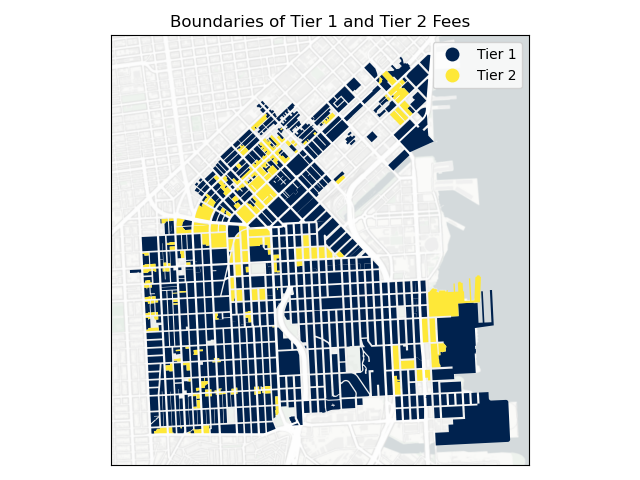
\includegraphics[scale=.8]{rdd/tier1_tier2_boundaries.png}
    \caption{RDD boundaries between fees.}
    \label{fig:tier1_tier2_boundaries}
\end{figure}

The boundaries can be viewed as discontinuities in a sharp regression discontinuity design. Instead of estimating the partial effect of the treatment D, I will estimate the average treatment effect of the higher fee F at a discontinuity. The treatment F is determined by:

\begin{equation}
F = \sum_{c \in C} I[(c^{min}_{lat} <= x_{lat} <= c^{max}_{lat}) \cap (c^{min}_{lon} <= x_{lon} <= c^{max}_{lon})]
\end{equation}

where C is a set of tuples $c:=(c^{min}_{lat}$, $c^{max}_{lat}$, $c^{min}_{lon} $, $c^{max}_{lon}$) of latitude and longitude coordinates that demarcate the boundaries of each rectangle where a higher fee is charged. Because these boundaries are non-overlapping, $F \in \{0, 1\}$. This RDD has two forcing variables $x_{lat}$ and $x_{lon}$ that determine the treatment.

The average treatment effect of F is defined as:
\begin{equation}
\tau_{c} \equiv \mathbb{E}[y_{1} - y_{0} \bigg| I(\exists c \in C \text{ s.t. } x_{lat} \in \{c^{min}_{lat}, c^{max}_{lat}\}, x_{lon} \in \{c^{min}_{lon}, c^{max}_{lon}\}) ]
\end{equation}

where $y_1$ and $y_0$ are the potential outcomes under treatment and control.

Though, in principle, there are two forcing variables $x_{lat}$ and $x_{lon}$, we can simplify the problem to one with a single forcing variables $x^{d}$ which denotes the Euclidean distance from the nearest boundary. This simplification preserves the physical sense in which a parcel can be near a boundary.

Now we can view the treatment as a binary treatment of applying the higher fee. To simplify the analysis, I use a 2014 cross-section of the panel dataset and let the outcome be the number of homes built on that parcel between 2014 and 2023. I model the outcome Y, the number of homes built per parcel, with local log-linear regression:

\begin{equation}
Y_i \sim {Poisson(\mu_i)}
\end{equation}

with 
\begin{equation}
log(\mu_i) = \alpha + \tau F_i + \beta_1 x^{d}_{i} + \gamma_1 (x^{d}_{i} \times F_i) + \sum{r_{ij}\beta_j}
\end{equation}

for observations $i$ where $x^{d}_{i}$ < h, where h is some threshold greater than zero. The covariates $r_{ij}$ reflect additional regressors.

Notably, the dataset is zero-inflated, and Y has a mean of 0.37 and variance of 52.4, so the Poisson assumption fails for this log-linear model, but I will correct for overdispersion later in the standard errors.

\begin{figure}[hbt]
    \centering
    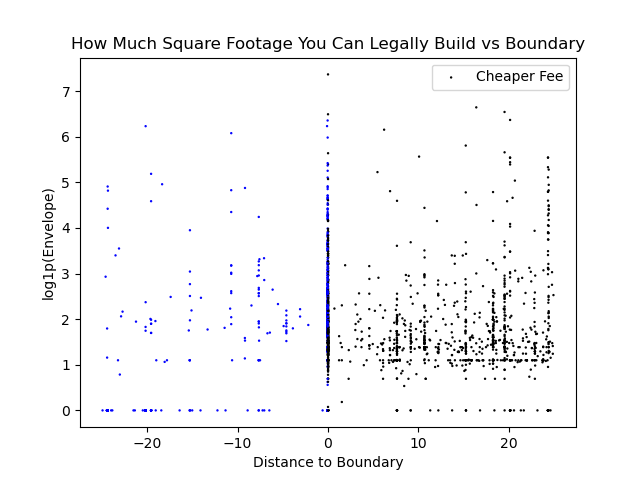
\includegraphics[scale=.8]{rdd/Envelope_boundary.png}
    \caption{RDD Boundary versus Known Compounding Treatment, Buildable Envelope.}
    \label{fig:Envelope_boundary}
\end{figure}

The boundaries reflect historical contingencies regarding when certain parcels were upzoned. Comparing parcels on either side of the border reflects fairly similar parcels for most variables. For example, a histogram breaking down the distribution of parcels with Office/Commercial Zoning is provided in \textbf{Figure \ref{fig:office_zoning_boundary}}. However, there is known compounding treatment because these neighborhoods were selected to receive additional upzoning, which is why they recieve higher fees. Evidence of these compounding treatments is provided in \textbf{Figure \ref{fig:Envelope_boundary}}. Additionally, certain applications of the higher residential impact fee are coextensive with higher impact fees on commercial development. Thus, I cannot assume all covariates vary continuously along the discontinuity; rather, I must include variables that are a function of zoning as additional regressors and indicators for higher commercial impact fees.

\begin{figure}[hbt]
    \centering
    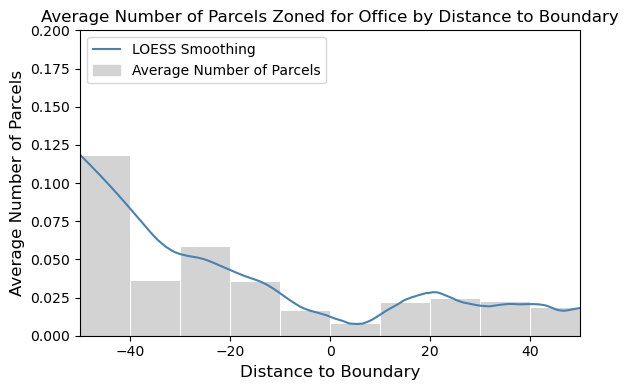
\includegraphics[scale=.8]{rdd/office_zoning_boundary.png}
    \caption{RDD Boundary versus Important Predictor, Office Zoning.}
    \label{fig:office_zoning_boundary}
\end{figure}

\subsubsection{Results}

With h=10 meters, I use forward stepAIC to select a log-linear model that minimizes AIC and it converges after nine steps. The estimated effect of F and other model summary statistics are presented in \textbf{Table \ref{tab:pois.results}}. The rsq.kl statistic is 0.65, which implies this model explains 65\% of the uncertainty in the dataset. After correcting for the dispersion parameter estimate of 1.47, the treatment variable F remains statistically significant with a p-value that's significant at the $\alpha=0.05$ level. The effect of $F$ on the log means-ratio is estimated to be -7.838, which implies that the effect of $F$ on the means-ratio amounts to orders of magnitude reductions in the rate of homes built. However, the confidence interval ranges widely on the means-ratio scale, from 0.00001 to 0.16, so the effect is not estimated precisely. At the upper-end of that bound, F is associated with an 84\% reduction in the rate of homes built per parcel. This seems remarkably more dramatic than one would anticipate.

\begin{table}[!htbp] \centering 
  \caption{Log-Linear Model Summary} 
  \small{Model also includes nine main effects omitted below.}
  \label{tab:pois.results} 
\begin{tabular}{@{\extracolsep{0pt}}rlc } 
\\[-1.8ex] & 95\% CI for Means-Ratio & P-Value \\ 
\hline \\[-1.8ex] 
  \textbf{F} & [-13.8094, -1.8673] &  0.010 \\

 \hline \\[-1.8ex] 
Observations & 1165 \\ 
AIC & 989.6 \\ 
$R^2_{kl}$ & 0.653 \\ 
\hline 
\end{tabular} 
\end{table} 

As a robustness check I tried varying h, the bandwidth that determines how local the regression is. The results of the analysis hinge dramatically on the choice of h, which implies the analysis is not robust to errors in misspecification of h. I chose a small h of 10 meters because doing so resolves concerns regarding how to estimate the slope of the response curve on each boundary point separately, a non-trivial task. Because I have a fairly large sample of n=1,165 observations with h=10, the small h is justifiable on grounds of minimizing bias.

I considered whether outliers were determinitive. But while the three outliers, as indicated by their Cook's distance, have a large effect on the fitted model, these three outliers are clearly valid data points; they only have large cook's distances because they are parcels that are developed into large apartments, and so their residuals are larger because these are unique parcels.

\begin{table}[hbt]
\centering
\setlength{\tabcolsep}{10pt} 
\caption{Robustness check on h}
\label{table:robust.h}
\begin{tabular}{|c|c|c|c|}
\hline
h & remaining sample size m & estimated effect & p-value \\
\hline
150 & 6046 & 0.81 & 2.2e-10 \\
125 & 5551 & 0.81 & 3.5e-10 \\
100 & 4905 & 1.22 & 4.0e-19 \\
75 & 4206 & 1.38  & 1.1e-18 \\
50 & 3221 & 1.35 & 6.6e-14 \\
25 & 2059 & 1.70 & 3.4e-09 \\
\hline
\end{tabular}
\end{table}


I performed another robustness check where I shifted the border so that parcels in the control group were assigned to the treatment if they were within k meters of the boundary, for k in (20, 25, 30, 35, 40, 45, 50). Spoofing the boundary in this way did change the results, but eventually flipped the sign and became significant again. See \textbf{Table \ref{tab:robust.spoof.k}} for the results of this experiment. P-values again are corrected for overdispersion.

\begin{table}[hbpt]
\centering
\caption{Placebo boundary robustness check}
\setlength{\tabcolsep}{10pt} 
\begin{tabular}{|c|c|c|}
\hline
k meters shifted & estimated effect & p-value \\
\hline
20 & 0.08070861 & 0.5660321 \\
25 & -0.7007796 & \(4.078483 \times 10^{-9}\) \\
30 & -0.394945 & \(0.001287085\) \\
35 & -0.6506453 & \(3.814174 \times 10^{-7}\) \\
40 & -0.8812792 & \(4.114295 \times 10^{-11}\) \\
45 & -1.088446 & \(2.481949 \times 10^{-15}\) \\
50 & -1.308117 & \(6.133475 \times 10^{-20}\) \\
\hline
\end{tabular}
\end{table}
\label{tab:robust.spoof.k}

These robustness checks demonstrate that the model is finnicky and not robust to perturbations in assumptions. This suggests that less confidence should be placed in the estimated effect for $F$. 

\section{Conclusion}

In all, the instrumental variable analysis was inconclusive, perhaps due to the limited number of accidental fires. In comparison, the RDD analysis was relatively more powerful and provides an bound that increasing fees by 1.2\% reduces the rate of homebuilding by at least 85\%. However, the RDD analysis is not robust to perturbations in how the model is specified, which implies that additional work may be necessary to improve the model.

For example, future work could extend the RDD model to be a local hurdle model wherein the probability of development occurring at all is modelled as a bernoulli and then the units built, conditioned on development occuring, is modelled as a negative binomial. This would improve the fit and ameliorate some of the extreme residuals found for the local log-linear regression. Furthermore, an analysis of spatial autocorrelation of errors is strictly speaking necessary to demonstrate that the assumptions of the model hold. Correcting for these autocorrelations, however, is very difficult.\cite{wooldridge2010econometric}

Future work notwithstanding, this report makes major strides in answering these questions first by creating a novel panel dataset for future research; second by proposing a novel way to impute data on construction costs; and third by proposing an innovative geospatial RDD analysis that shows promise in answering key questions regarding the supply effects of housing legislation.


\printbibliography

\clearpage
\section*{Appendix}
\begin{verbatim}
All code is available on my public github repository, here: https://github.com/sdamerdji/dissertation
\end{verbatim}
\end{document}

